\chapter{Hardware Design} \label{ch:HwDesign}

\section*{Version}
\begin{table}[h]
	\centering
	\begin{tabularx}{\textwidth - 2cm}{|l|l|l|X|}
	\hline
	Dato	& Version	& Initialer & Ændring	\\ \hline
	30. marts & 1 & PKP & PSoC Master use case diagram og klassebeskrivelser tilføjet.\\ \hline
	30. marts & 2 & MHG & I2C Protokol og design af Aktuator. \\ \hline
	8. april & 3 & MHG & Mindre rettelser i Aktuatordesign. \\ \hline
	10. april & 4 & MHG & Skrevet det sidste (varmelegeme) design i aktuator blokken. \\\hline
	23. april & 5 & MHG & Lavet mindre rettelser i et par diagrammer. \\\hline
	27. april & 6 & MHG & Skrevet design for Strømforsyning. \\\hline
	27. april & 7 & PKP & Design for PSoC master rettet.	\\\hline
	1. maj & 8 & MHG & Skrevet design for Slave Jordfugt. \\\hline
	13. maj & 9 & PKP & \IIC protokol opdateret med ny temperatursensor og PSoC Master funktionsbeskrivelser opdateret. \\\hline
	21. maj & 10 & LBS & Tilføjet breakoutboard afsnit. \\\hline
	\end{tabularx}
\end{table}

\clearpage
\section{\IIC Protokol} \label{sec:I2C_protokol}
Dette afsnit omhandler kommunikationen mellem alle \IIC kommunikerende komponenter i projektet.

\subsection{Temp-/Luftfugtighedssensor}
Information om Temperatur- og Luftfugtighedssensor er fundet under komponentens datasheet. Bilag 004 \cite{lib:TempHum_I2C}.

%Slave Temp-/Luftfugtihed
\begin{table}[h]
\centering
\begin{tabularx}{0.6\textwidth}{| X | X |} 			\hline
\textbf{Slave:} 		& Temp-/Luftfugtighed		\\ \hline
\textbf{Adresse:}		& 0x27						\\ \hline
\textbf{Bemærkninger:}	& scl: 100-400 kHz			\\ \hline
\end{tabularx}
\caption{\IIC Oplysninger for Temp-/Luftfugtigedhedssensor}
\label{tbl:I2CTempLuftOplysninger}
\end{table}


Når der skal læses data fra sensoren, sker det jf. Figur \ref{fig:I2CTempLuftProtokol}, fundet under Bilag 004 side 2 \cite{lib:TempHum_I2C}.


\begin{figure}[h]
\centering
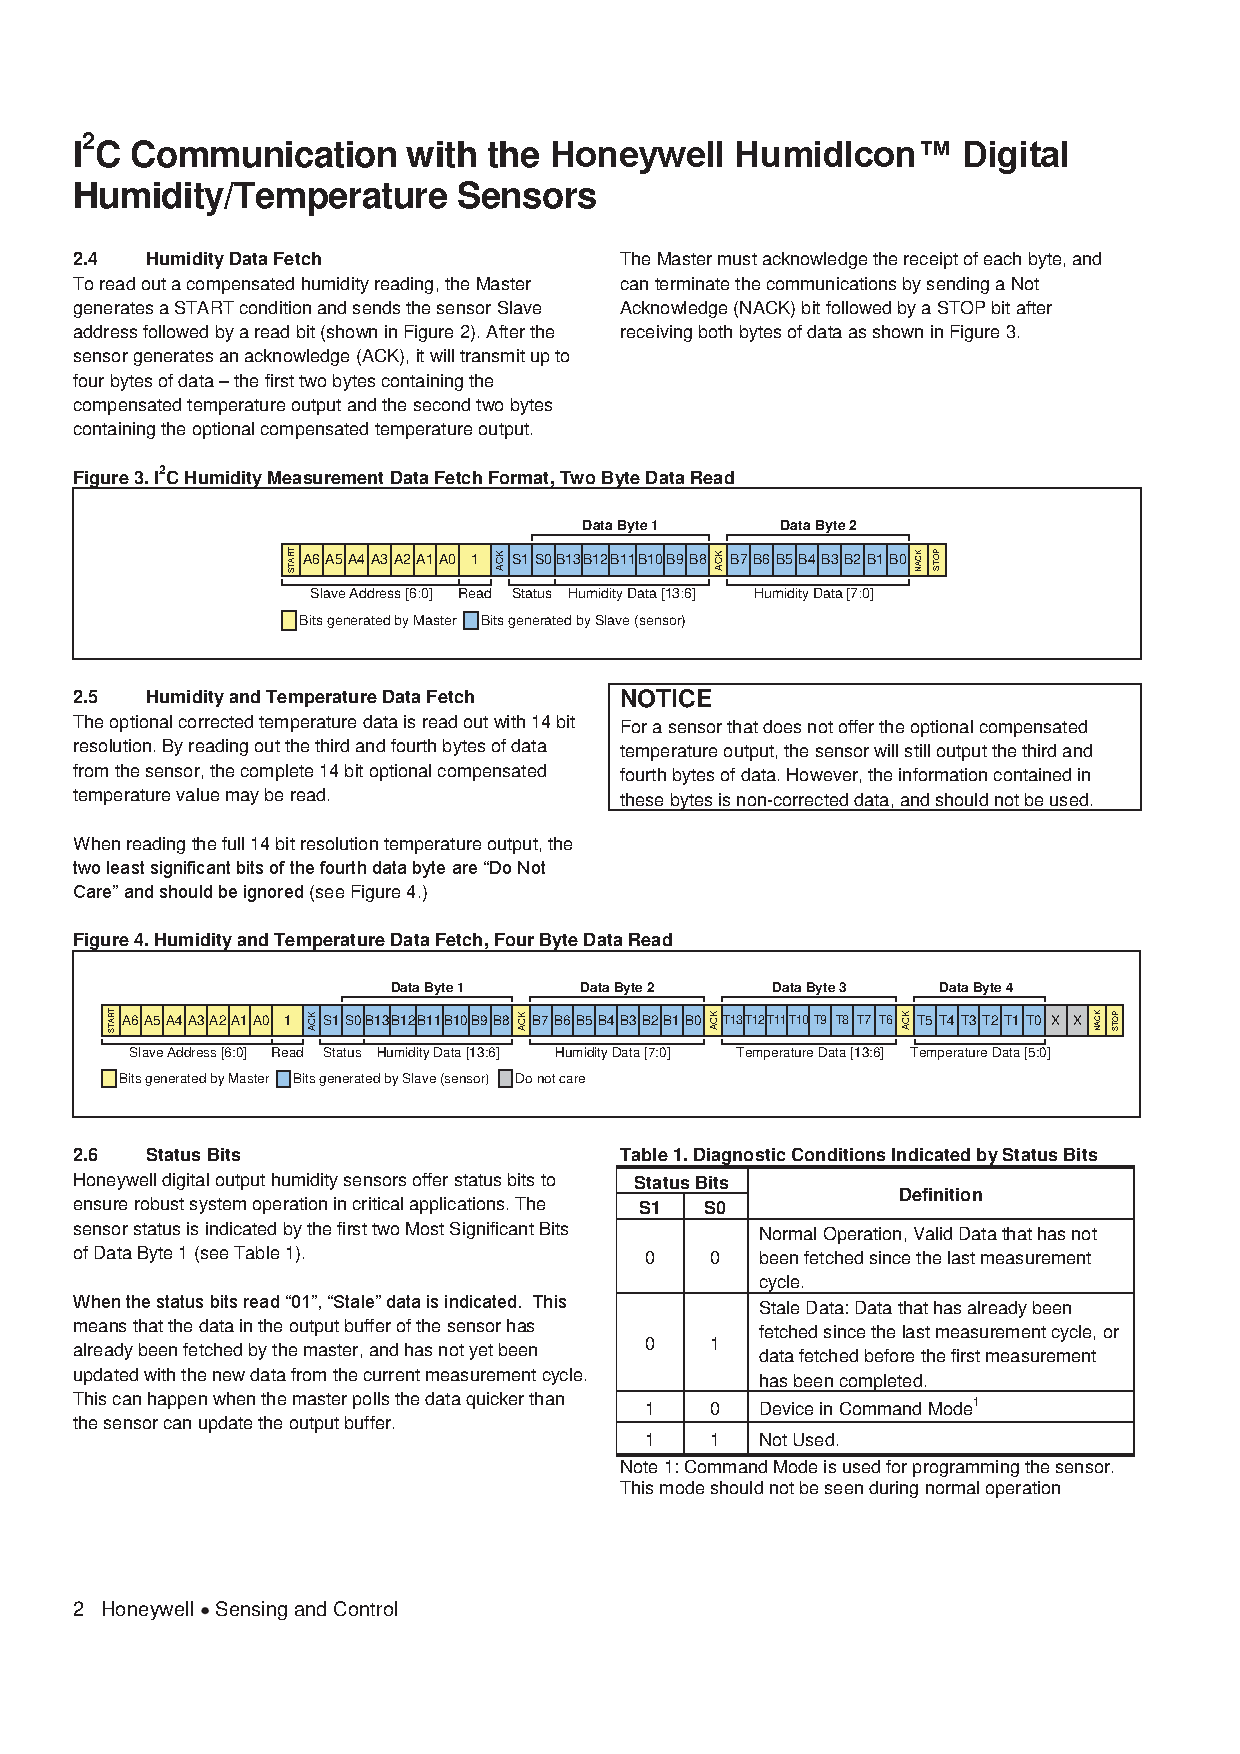
\includegraphics[width=\textwidth - 1 cm, clip=true, trim=48 319 55 471]{../fig/I2CTempLuftProtokol.pdf}
\caption{\IIC protokol for Temp-/Luftfugtighedssensor}
\label{fig:I2CTempLuftProtokol}
\end{figure}

\clearpage

\subsection{Slave Aktuator}
%Slave Aktuator
\begin{table}[h]
\centering
\begin{tabularx}{0.6\textwidth}{| X | X |} 			\hline
\multicolumn{2}{ | l | }{\textbf{Adresse:} 0x42} 	\\ \hline
\textbf{Kommando} 		& \textbf{Beskrivelse}		\\ \hline
WriteAdjustWindow		& Åbning/Lukning af vindue	\\ \hline
WriteAdjustHeat			& Tænd/Sluk for varme		\\ \hline
WriteAdjustVentilation	& Juster ventilation		\\ \hline
WriteAdjustIrrigation	& Juster vanding			\\ \hline
ReadStatus				& Anmodning om status		\\ \hline
\end{tabularx}
\caption{\IIC Kommandoer for Slave Aktuator}
\label{tbl:I2CAktuatorKommandoer}
\end{table}



%WriteAdjustWindow
\begin{table}[h]
\centering
\begin{tabularx}{0.6\textwidth}{| >{\centering\arraybackslash}X | >{\centering\arraybackslash}X | >{\centering\arraybackslash}X | >{\centering\arraybackslash}X | >{\centering\arraybackslash}X | >{\centering\arraybackslash}X | >{\centering\arraybackslash}X | >{\centering\arraybackslash}X |}	\hline
W7 & W6 & W5 & W4 & W3 & W2 & W1 & W0				\\ \hline
\multicolumn{2}{ | l | }{0x0} 						&
\multicolumn{2}{  l | }{Don't Cares}				&
\multicolumn{4}{  l | }{Position for vindue,}
\\
\multicolumn{2}{ | l | }{} 							&
\multicolumn{2}{  l | }{}							&
\multicolumn{4}{  l | }{0x0 = lukket, 0xF = åben}
\\ \hline
\end{tabularx}
\caption{\IIC Kommando WriteAdjustWindow}
\label{tbl:I2CAktuatorKommandoWriteAdjustWindow}
\end{table}



%WriteAdjustHeat
\begin{table}[h]
\centering
\begin{tabularx}{0.6\textwidth}{| >{\centering\arraybackslash}X | >{\centering\arraybackslash}X | >{\centering\arraybackslash}X | >{\centering\arraybackslash}X | >{\centering\arraybackslash}X | >{\centering\arraybackslash}X | >{\centering\arraybackslash}X | >{\centering\arraybackslash}X |}	\hline
H7 & H6 & H5 & H4 & H3 & H2 & H1 & H0				\\ \hline
\multicolumn{2}{ | l | }{0x1} 						&
\multicolumn{3}{  l | }{Don't Care}					&
\multicolumn{3}{  l | }{Tænd/Sluk}
\\
\multicolumn{2}{ | l | }{} 							&
\multicolumn{3}{  l | }{}							&
\multicolumn{3}{  l | }{varmelegeme,}
\\
\multicolumn{2}{ | l | }{} 							&
\multicolumn{3}{  l | }{}							&
\multicolumn{3}{  l | }{0x0 = off, 0x7 = on}
\\ \hline
\end{tabularx}
\caption{\IIC Kommando WriteAdjustHeat}
\label{tbl:I2CAktuatorKommandoWriteAdjustHeat}
\end{table}

\clearpage

%WriteAdjustVentilation
\begin{table}[h]
\centering
\begin{tabularx}{0.6\textwidth}{| >{\centering\arraybackslash}X | >{\centering\arraybackslash}X | >{\centering\arraybackslash}X | >{\centering\arraybackslash}X | >{\centering\arraybackslash}X | >{\centering\arraybackslash}X | >{\centering\arraybackslash}X | >{\centering\arraybackslash}X |}	\hline
V7 & V6 & V5 & V4 & V3 & V2 & V1 & V0				\\ \hline
\multicolumn{2}{ | l | }{0x2} 						&
\multicolumn{3}{  l | }{Don't Care}					&
\multicolumn{3}{  l | }{Tænd/Sluk}
\\
\multicolumn{2}{ | l | }{} 							&
\multicolumn{3}{  l | }{}							&
\multicolumn{3}{  l | }{ventilation,}
\\
\multicolumn{2}{ | l | }{} 							&
\multicolumn{3}{  l | }{}							&
\multicolumn{3}{  l | }{0x0 = off, 0x7 = on}
\\ \hline
\end{tabularx}
\caption{\IIC Kommando WriteAdjustVentilation}
\label{tbl:I2CAktuatorKommandoWriteAdjustVentilation}
\end{table}



%WriteAdjustIrrigation
\begin{table}[h]
\centering
\begin{tabularx}{0.6\textwidth}{| >{\centering\arraybackslash}X | >{\centering\arraybackslash}X | >{\centering\arraybackslash}X | >{\centering\arraybackslash}X | >{\centering\arraybackslash}X | >{\centering\arraybackslash}X | >{\centering\arraybackslash}X | >{\centering\arraybackslash}X |}	\hline
I7 & I6 & I5 & I4 & I3 & I2 & I1 & I0				\\ \hline
\multicolumn{2}{ | l | }{0x3} 						&
\multicolumn{6}{  l | }{Værdi for pins til vanding,}
\\
\multicolumn{2}{ | l | }{} 							&
\multicolumn{6}{  l | }{I5: nr. 6 – I0: nr. 1,}
\\
\multicolumn{2}{ | l | }{} 							&
\multicolumn{6}{  l | }{1 = on, 0 = off}
\\ \hline
\end{tabularx}
\caption{\IIC Kommando WriteAdjustIrrigation}
\label{tbl:I2CAktuatorKommandoWriteAdjustIrrigation}
\end{table}



%ReadStatus
\begin{table}[!h]
\begin{tabularx}{\textwidth}{| >{\centering\arraybackslash}X | >{\centering\arraybackslash}X | >{\centering\arraybackslash}X | >{\centering\arraybackslash}X | >{\centering\arraybackslash}X | >{\centering\arraybackslash}X | >{\centering\arraybackslash}X | >{\centering\arraybackslash}X | >{\centering\arraybackslash}X | >{\centering\arraybackslash}X | >{\centering\arraybackslash}X | >{\centering\arraybackslash}X | >{\centering\arraybackslash}X | >{\centering\arraybackslash}X | >{\centering\arraybackslash}X | >{\centering\arraybackslash}X |}	\hline
W3 & W2 & W1 & W0 & H2 & H1 & H0 & V2 & V1 & V0 & I5 & I4 & I3 & I2 & I1 & I0				\\ \hline
\multicolumn{4}{ | l | }{Position for vindue,} 			&
\multicolumn{3}{  l | }{Status for}						&
\multicolumn{3}{  l | }{Status for}						&
\multicolumn{6}{  l | }{Status for pins til vanding,}
\\
\multicolumn{4}{ | l | }{0x0 = lukket,} 				&
\multicolumn{3}{  l | }{Varmelegeme,}					&
\multicolumn{3}{  l | }{ventilation,}					&
\multicolumn{6}{  l | }{I5: nr. 6 – I0: nr. 1,}	
\\
\multicolumn{4}{ | l | }{0xF = åben} 					&
\multicolumn{3}{  l | }{1 = on,}						&
\multicolumn{3}{  l | }{0x0 = off,}						&
\multicolumn{6}{  l | }{1 = on,}
\\
\multicolumn{4}{ | l | }{} 								&
\multicolumn{3}{  l | }{0 = off}						&
\multicolumn{3}{  l | }{0x7 = on}						&
\multicolumn{6}{  l | }{0 = off}					
\\ \hline
\end{tabularx}
\caption{\IIC Kommando ReadStatus}
\label{tbl:I2CAktuatorKommandoReadStatus}
\end{table}

\clearpage
\section{PSoC Master} \label{sec:PSoC_Master_design}

På Figur \ref{fig:Master_PSoC_klassediagram} ses klassediagrammet for Master PSoC. Der er blevet designet 4 klasser der håndterer hver sin del af arbejdet, som masteren skal udføre. Der er valgt to boundaryklasser, som håndterer kommunikation over hhv. UART og \IIC. Udover dette er der en domæneklasse, som indeholder alle de målte dataværdier, der er modtaget af sensorerne. 

\begin{figure}[h]
\centering 
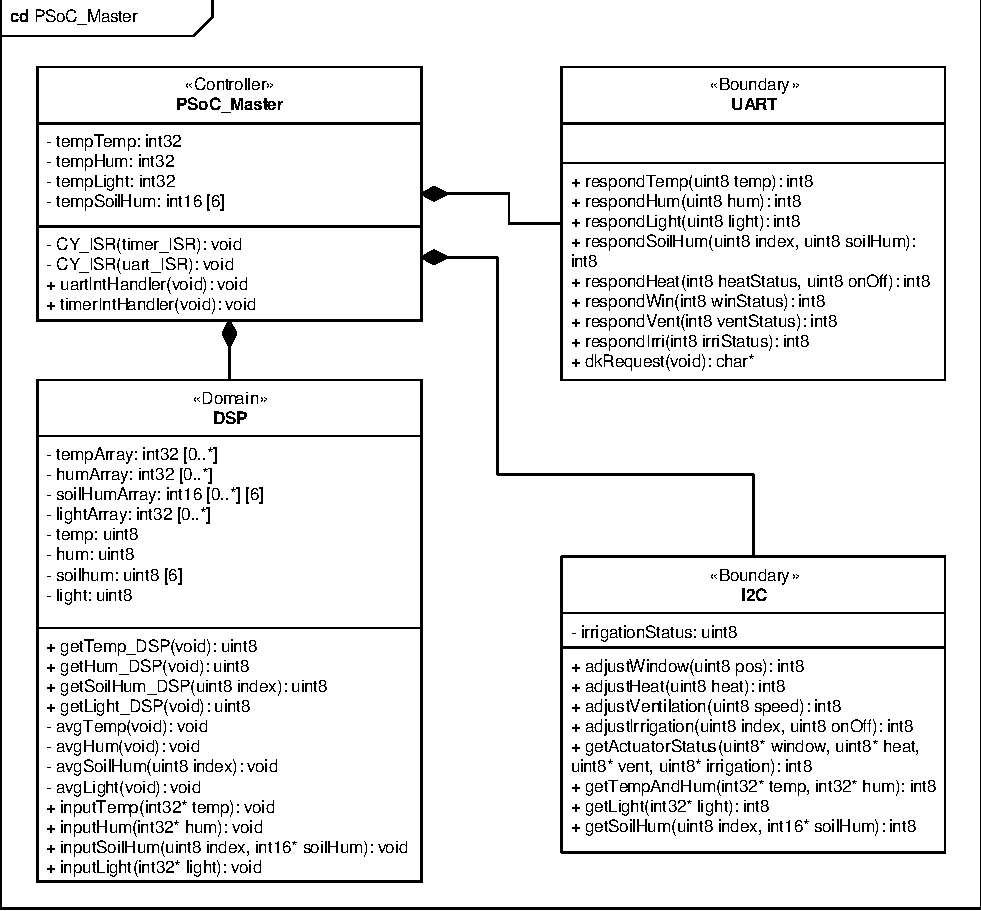
\includegraphics[width={\textwidth}, trim=0 0 0 0, clip=true] {../fig/cd_PSoC_master.pdf}
\caption{Klassediagram for Master PSoC}
\label{fig:Master_PSoC_klassediagram}
\end{figure}

\clearpage

\subsection{Klassebeskrivelser}

%++++++++++++ Controller PSoC Master klassen ++++++++++++++
\subsubsection{Controllerklasse PSoC\_Master}

\textbf{Attributter}

\begin{table}[h]
\begin{tabularx}{\textwidth}{| >{\raggedright\arraybackslash}X | >{\raggedright\arraybackslash}X | >{\raggedright\arraybackslash}p{10 cm} |} \hline
\texttt{tempTemp} & \texttt{int32} & Midlertidig variabel til opbevaring af temperatur. \\\hline
\texttt{tempHum} & \texttt{int32} & Midlertidig variabel til opbevaring af luftfugtighed. \\\hline
\texttt{tempLight} & \texttt{int32} & Midlertidig variabel til opbevaring af lysintensitet. \\\hline
\texttt{tempSoilHum} & \texttt{int16} & Midlertidig variabel til opbevaring af jordfugtighed. \\\hline
\end{tabularx}
\caption{Attributter for klassen PSoC\_Master}
\label{table:PSoC_Master_attributter}
\end{table}

\textbf{Metoder}

%========================= CY_ISR(timer_ISR) ==============

\begin{table}[h]
\begin{tabularx}{\textwidth}{| >{\raggedright\arraybackslash}p{2.5 cm} | >{\raggedright\arraybackslash}X |} \hline
Prototype & \texttt{void CY\_ISR(timer\_ISR)} \\\hline
Parametre & \texttt{timer\_ISR} \newline Vector for den givne interrupt servicerutine. \\\hline
Returværdi & - \\\hline
Beskrivelse & Denne interrupt service rutine bliver kaldt, når en ønsket tidsperiode er forløbet. Rutinen kalder metoder i boundaryklassen \IIC, der varetager indhentning af data fra sensorer.  \\\hline
\end{tabularx}
\caption{CY\_ISR(timer\_ISR)}
\label{table:CY_ISR(timer_ISR)}
\end{table}

%========================= CY_ISR(uart_ISR) ==============

\begin{table}[h]
\begin{tabularx}{\textwidth}{| >{\raggedright\arraybackslash}p{2.5 cm} | >{\raggedright\arraybackslash}X |} \hline
Prototype & \texttt{void CY\_ISR(uart\_ISR)} \\\hline
Parametre & \texttt{uart\_ISR} \newline 
Vector for den givne interrupt servicerutine. \\\hline
Returværdi & - \\\hline
Beskrivelse & Denne interrupt service rutine bliver kaldt, når der modtages noget på UART fra DevKit8000. Rutinen kalder metoder i boundaryklasserne \IIC og UART. Formålet med interrupten er at håndtere forskellige typer af forespørgsler. \\\hline
\end{tabularx}
\caption{CY\_ISR(uart\_ISR)}
\label{table:CY_ISR(uart_ISR)}
\end{table}

%========================= FLERE UART FUNKTIONER ==============

\newpage

\subsubsection{Boundaryklasse UART}
%+++++++++++++++++++++++++ Boundary UART ++++++++++++++++++++
\textbf{Metoder}

%========================= respondTemp ==============

\begin{table}[h]
\begin{tabularx}{\textwidth}{| >{\raggedright\arraybackslash}p{2.5 cm} | >{\raggedright\arraybackslash}X |} \hline
Prototype & \texttt{int8 respondTemp(uint8 temp)} \\\hline
Parametre & \texttt{uint8 temp} \newline
Den nyeste midlede temperatur hentet fra domæneklassen DSP. 
 \\\hline
Returværdi & \texttt{int8} \newline
Er denne værdi nul er der blevet returneret en gyldig værdi. Hvis værdien er -1 er der blevet returneret ’XT’ over UART. \\\hline
Beskrivelse & Hvis parameter værdien ligger inden for decimalværdien 1-200 (begge inklusive), skal metoden sende en char ’T’, efterfulgt af temp parameteren, over UART. Er værdien er lig nul, skal metoden sende strengen ”XT".   \\\hline
\end{tabularx}
\caption{respondTemp}
\label{table:respondTemp}
\end{table}

%========================= respondHum ==============

\begin{table}[h]
\begin{tabularx}{\textwidth}{| >{\raggedright\arraybackslash}p{2.5 cm} | >{\raggedright\arraybackslash}X |} \hline
Prototype & \texttt{ int8 respondHum(uint8 hum)} \\\hline
Parametre & \texttt{uint8 hum} \newline
Den nyeste midlede luftfugtighed hentet fra domæneklassen DSP. 
 \\\hline
Returværdi & \texttt{int8} \newline
Er denne værdi nul er der blevet returneret en gyldig værdi. Hvis værdien er -1 er der blevet returneret ’XA’ over UART. \\\hline
Beskrivelse & Hvis parameter værdien ligger inden for decimalværdien 1-100 (begge inklusive), skal metoden sende en char ’A’, efterfulgt af hum parameteren, over UART. Hvis værdien er lig nul, skal metoden sende strengen ”XA".    \\\hline
\end{tabularx}
\caption{respondHum}
\label{table:respondHum}
\end{table}

%========================= respondLight ==============

\begin{table}[h]
\begin{tabularx}{\textwidth}{| >{\raggedright\arraybackslash}p{2.5 cm} | >{\raggedright\arraybackslash}X |} \hline
Prototype & \texttt{int8 respondLight(uint8 light)} \\\hline
Parametre & \texttt{uint8 light} \newline
Den nyeste midlede lysintensitet hentet fra domæneklassen DSP. 
 \\\hline
Returværdi & \texttt{int8} \newline
Er denne værdi nul er der blevet returneret en gyldig værdi. Hvis værdien er -1 er der blevet returneret ’XL’ over UART.\\\hline
Beskrivelse & Hvis parameter værdien ligger inden for decimalværdien 1-100 (begge inklusive), skal metoden sende en char ’L’ efterfulgt af light parameteren over UART. Hvis værdien er lig nul, skal metoden sende strengen ”XL".     \\\hline
\end{tabularx}
\caption{respondLight}
\label{table:respondLight}
\end{table}

%========================= respondSoilHum ==============

\begin{table}[h]
\begin{tabularx}{\textwidth}{| >{\raggedright\arraybackslash}p{2.5 cm} | >{\raggedright\arraybackslash}X |} \hline
Prototype & \texttt{int8 respondSoilHum(uint8 index, uint8 soilHum)} \\\hline
Parametre & \texttt{uint8 soilHum} \newline
Den nyeste midlede jordfugtighed hentet fra domæneklassen DSP. \newline
\texttt{uint8 index} \newline
Indexet fortæller hvilket sensornummer der svares fra. \\\hline
Returværdi & \texttt{int8} \newline
Er denne værdi nul er der blevet returneret en gyldig værdi. Hvis værdien er -1 er der blevet returneret ’XS’ over UART.\\\hline
Beskrivelse & Hvis parameter værdien ligger inden for decimalværdien 1-10 (begge inklusive), skal metoden sende en char ’S’, efterfulgt af index og soilHum parametrene over UART. Hvis værdien for soilHum er lig nul, skal metoden sende strengen ”XS". \\\hline
\end{tabularx}
\caption{respondSoilHum}
\label{table:respondSoilHum}
\end{table}

%========================= respondHeat ==============

\begin{table}[h]
\begin{tabularx}{\textwidth}{| >{\raggedright\arraybackslash}p{2.5 cm} | >{\raggedright\arraybackslash}X |} \hline
Prototype & \texttt{int8 respondHeat(uint8 heatStatus, uint8 On)} \\\hline
Parametre & \texttt{uint8 heatStatus} \newline
Returværdien fra funktionen adjustHeat i boundaryklassen \IIC; fortæller om kommunikationen over \IIC er gået godt. \newline
\texttt{uint8 On} \newline
Returværdi til UART afhængig af hvilken kommando, der blev kaldt. 0 = off, 0 != on.
 \\\hline
Returværdi & \texttt{int8} \newline
Er denne værdi nul er kommunikationen over \IIC gennemført. Hvis værdien er
-1 er der blevet returneret en værdi tilsvarene requesten fra DevKit8000 over UART (se UART protokol side \pageref{UART_Protokol}) og der er sket en fejl i kommunikationen over \IIC.
\\\hline
Beskrivelse & Hvis parameter værdien er lig nul, sendes en char tilsvarene requesten over UART. Hvis værdien er lig -1, sendes sendes en tilsvarene fejlmeddelelse. \\\hline
\end{tabularx}
\caption{respondHeat}
\label{table:respondHeat}
\end{table}

%========================= respondWin ==============

\begin{table}[h]
\begin{tabularx}{\textwidth}{| >{\raggedright\arraybackslash}p{2.5 cm} | >{\raggedright\arraybackslash}X |} \hline
Prototype & \texttt{int8 respondWin(int8 winStatus)} \\\hline
Parametre & \texttt{int8 winStatus} \newline
Returværdien fra funktionen adjustWin i boundaryklassen \IIC. Fortæller om kommunikationen via. \IIC til vinduesaktuatoren er forløbet godt.  
 \\\hline
Returværdi & \texttt{int8} \newline
Er denne værdi nul er kommunikationen over \IIC gennemført. Hvis værdien er -1 er der blevet returneret ’XK’ over UART og der er sket en fejl i kommunikationen over \IIC.\\\hline
Beskrivelse & Hvis parameter værdien er lig nul, sendes en char ’K’ over UART. Hvis værdien er lig -1, sendes strengen ”XK". \\\hline
\end{tabularx}
\caption{respondWin}
\label{table:respondWin}
\end{table}

%========================= respondVent ==============

\begin{table}[h]
\begin{tabularx}{\textwidth}{| >{\raggedright\arraybackslash}p{2.5 cm} | >{\raggedright\arraybackslash}X |} \hline
Prototype & \texttt{int8 respondVent(int8 ventStatus)} \\\hline
Parametre & \texttt{int8 ventStatus} \newline
Returværdien fra funktionen adjustVent i boundaryklassen \IIC. Fortæller om kommunikationen via \IIC til ventilatoraktuatoren er forløbet uden problemer.   
 \\\hline
Returværdi & \texttt{int8} \newline
Er denne værdi 0, er kommunikationen over \IIC gennemført. Hvis værdien er 
-1 er der blevet returneret ’XV’ over UART og der er sket en fejl i kommunikationen over \IIC.
\\\hline
Beskrivelse & Hvis parameterværdien er lig nul, sendes en char ’V’ over UART, hvilket indikerer at det er gået godt. Hvis værdien er lig -1, sendes strengen ”XV". \\\hline
\end{tabularx}
\caption{respondVent}
\label{table:respondVent}
\end{table}

%========================= respondIrri ==============

\begin{table}[h]
\begin{tabularx}{\textwidth}{| >{\raggedright\arraybackslash}p{2.5 cm} | >{\raggedright\arraybackslash}X |} \hline
Prototype & \texttt{int8 respondIrri(int8 irriStatus)} \\\hline
Parametre & \texttt{int8 irriStatus} \newline
Returværdien fra funktionen adjustIrrigation i boundaryklassen \IIC. Fortæller om kommunikationen via \IIC til irrigationsaktuatoren er forløbet uden problemer.   
 \\\hline
Returværdi & \texttt{int8} \newline
Er denne værdi nul, er kommunikationen over \IIC gennemført. Hvis værdien er 
-1 er der blevet returneret ’XF’ over UART og der er sket en fejl i kommunikationen over \IIC.
\\\hline
Beskrivelse & Hvis parameterværdien er lig nul, sendes en char ’F’ over UART, hvilket indikerer at det er gået godt. Hvis værdien er lig 
-1, sendes strengen ”XF". \\\hline
\end{tabularx}
\caption{respondIrri}
\label{table:respondIrri}
\end{table}

\clearpage

%+++++++++++++++++++++++++ I2C klassen ++++++++++++++
\subsubsection{Boundaryklasse \IIC}

\textbf{Attributter}

\begin{table}[h]
\begin{tabularx}{\textwidth}{| >{\raggedright\arraybackslash}X | >{\raggedright\arraybackslash}X | >{\raggedright\arraybackslash}p{8 cm} |} \hline
Navn & Type & Beskrivelse \\\hline
\texttt{irrigationStatus} & \texttt{uint8} & Indeholder den aktuelle status for vandingsaktuatorer (tændt eller slukkede). Bit 0 – 5 er hhv. aktuatorerne fra 1 – 6. Nul betyder slukket og et betyder tændt. \\\hline
\end{tabularx}
\caption{Attributter for klassen \IIC}
\label{table:IIC_attributter}
\end{table}

\textbf{Metoder}

%========================= adjustWindow ==============

\begin{table}[h]
\begin{tabularx}{\textwidth}{| >{\raggedright\arraybackslash}p{2.5 cm} | >{\raggedright\arraybackslash}X |} \hline
Prototype & \texttt{int8 adjustWindow(uint8 pos)} \\\hline
Parametre & \texttt{uint8 pos} \newline 
Den ønskede status for vinduet. Kan være hhv. 0xFF for åben og 0x00 for lukket. \\\hline
Returværdi & \texttt{int8} \newline
Er værdien 0, er kommunikation via \IIC gået godt. Hvis værdien er -1, er der sket en fejl. \\\hline
Beskrivelse & Metoden kan justere positionen for vinduet i drivhuset. Sender kommandoen ”WriteAdjustWindow” via \IIC bussen (se \IIC protokol på side \pageref{sec:I2C_protokol}). \\\hline
\end{tabularx}
\caption{adjustWindow}
\label{table:adjustWindow}
\end{table}

%========================= adjustHeat ==============

\begin{table}[h]
\begin{tabularx}{\textwidth}{| >{\raggedright\arraybackslash}p{2.5 cm} | >{\raggedright\arraybackslash}X |} \hline
Prototype & \texttt{int8 adjustHeat(uint8 heat)} \\\hline
Parametre & \texttt{uint8 heat} \newline 
Bestemmer intensiteten af varmen, 0x00 er ingen varme, 0xFF er fuld varme. \\\hline
Returværdi & \texttt{int8} \newline
Er værdien 0, er kommunikation via \IIC gået godt. Hvis værdien er -1, er der sket en fejl (se \IIC protokol på side \pageref{sec:I2C_protokol}). \\\hline
Beskrivelse & Slukker eller tænder for varmeaktuatoren. Sender kommandoen ”WriteAdjustHeat” via \IIC bussen (se \IIC protokol på side \pageref{sec:I2C_protokol}). \\\hline
\end{tabularx}
\caption{adjustHeat}
\label{table:adjustHeat}
\end{table}

%========================= adjustVentilation ==============

\begin{table}[h]
\begin{tabularx}{\textwidth}{| >{\raggedright\arraybackslash}p{2.5 cm} | >{\raggedright\arraybackslash}X |} \hline
Prototype & \texttt{int8 adjustVentilation(uint8 speed)} \\\hline
Parametre & \texttt{uint8 speed} \newline 
Beskriver ventilatoraktuatornes tilstand. 0x00 svarer til slukket og 0xFF svarer til fuld hastighed. \\\hline
Returværdi & \texttt{int8} \newline
Er værdien 0, er kommunikation via \IIC gået godt. Hvis værdien er -1, er der sket en fejl (se \IIC protokol på side \pageref{sec:I2C_protokol}). \\\hline
Beskrivelse & Slukker eller tænder for ventilation. Sender kommandoen ”WriteAdjustVentilation” via \IIC bussen (se \IIC protokol på side \pageref{sec:I2C_protokol}). \\\hline
\end{tabularx}
\caption{adjustVentilation}
\label{table:adjustVent}
\end{table}

%========================= adjustIrrigation ==============

\begin{table}[h]
\begin{tabularx}{\textwidth}{| >{\raggedright\arraybackslash}p{2.5 cm} | >{\raggedright\arraybackslash}X |} \hline
Prototype & \texttt{int8 adjustIrrigation(uint8 index, uint8 on)} \\\hline
Parametre & \texttt{uint8 index} \newline 
Indeksoperator for hvilken vandingsaktuator der skal aktiveres. Første = 0, sidste = 5. \newline
\texttt{uint8 on} \newline
Beskriver tilstanden for vandingsaktuatoren. 0x00 svarer til slukket og 0xFF svarer til tændt. \\\hline
Returværdi & \texttt{int8} \newline
Er værdien 0, er kommunikation via \IIC gået godt. Hvis værdien er -1, er der sket en fejl (se \IIC protokol på side \pageref{sec:I2C_protokol}). \\\hline
Beskrivelse & Slukker eller tænder for individuelle vandingsaktuatorer. Sender kommandoen ”WriteAdjustIrrigation” via \IIC bussen (se \IIC protokol på side \pageref{sec:I2C_protokol}). \\\hline
\end{tabularx}
\caption{adjustIrrigation}
\label{table:adjustIrri}
\end{table}

%========================= getActuatorStatus ==============

\begin{table}[h]
\begin{tabularx}{\textwidth}{| >{\raggedright\arraybackslash}p{2.5 cm} | >{\raggedright\arraybackslash}X |} \hline
Prototype & \texttt{int8 getActuatorStatus(uint8* window, uint8* heat, \newline uint8* vent, uint8* irrigation)} \\\hline
Parametre & \texttt{uint8* window} \newline 
Pointer til variable som status for vinduet skrives i. \newline
\texttt{uint8* heat} \newline
Pointer til variable som status for varmelegeme skrives i. \newline
\texttt{uint8 uint8* vent} \newline
Pointer til variable som status for ventilator skrives i. \newline
\texttt{uint8* irrigation} \newline
Pointer til variable som status for vandingsaktuatorer skrives i. \\\hline
Returværdi & \texttt{int8} \newline
Er værdien 0, er kommunikation via \IIC gået godt. Hvis værdien er -1, er der sket en fejl. \\\hline
Beskrivelse & Giver overblik over aktuatorslavens tilstand. Der henvises til \IIC protokollen på side \pageref{sec:I2C_protokol} for yderligere information. \\\hline
\end{tabularx}
\caption{getActuatorStatus}
\label{table:getActuatorStatus}
\end{table}

%========================= getTempAndHum ==============

\begin{table}[h]
\begin{tabularx}{\textwidth}{| >{\raggedright\arraybackslash}p{2.5 cm} | >{\raggedright\arraybackslash}X |} \hline
Prototype & \texttt{int8 getTempAndHum(int32* temp, int32* hum)} \\\hline
Parametre & \texttt{int32* temp} \newline 
Pointer til variabel, hvori ubehandlet temperaturdata i drivhuset skrives. \newline
\texttt{int32* hum} \newline
Pointer til variabel, hvori ubehandlet luftfugtighedsdata i drivhuset skrives. \newline \newline
Omregningsformel kan findes i databladet for sensoren. \cite{lib:TempHum_I2C} \\\hline
Returværdi & \texttt{int8} \newline
Er værdien 0, er kommunikation via \IIC gået godt. Hvis værdien er -1, er der sket en fejl. \\\hline
Beskrivelse & Metoden skriver ubehandlet data fra sensoren i to variable. Der henvises til \IIC protokollen på side \pageref{sec:I2C_protokol} og til sensorens datablad \cite{lib:TempHum_I2C} for yderligere information. \\\hline
\end{tabularx}
\caption{getTempAndHum}
\label{table:getTempAndHum}
\end{table}

%========================= getLight ==============

\begin{table}[h]
\begin{tabularx}{\textwidth}{| >{\raggedright\arraybackslash}p{2.5 cm} | >{\raggedright\arraybackslash}X |} \hline
Prototype & \texttt{int8 getLight(int32* light)} \\\hline
Parametre & \texttt{int32* light} \newline 
Pointer til variabel, hvori ubehandlet lysintensitetsdata i drivhuset skrives. \newline \newline
Omregningsformel kan findes i databladet for sensoren. \cite{lib:LightSens}. \\\hline
Returværdi & \texttt{int8} \newline
Er værdien 0, er kommunikation via \IIC gået godt. Hvis værdien er -1, er der sket en fejl. \\\hline
Beskrivelse & Metoden skriver ubehandlet data fra sensoren i en variabel. Der henvises til \IIC protokollen på side \pageref{sec:I2C_protokol} og til sensorens datablad \cite{lib:LightSens} for yderligere information. \\\hline
\end{tabularx}
\caption{getLight}
\label{table:getLight}
\end{table}

%========================= getSoilHum ==============

\begin{table}[h]
\begin{tabularx}{\textwidth}{| >{\raggedright\arraybackslash}p{2.5 cm} | >{\raggedright\arraybackslash}X |} \hline
Prototype & \texttt{uint8* getSoilHum(uint8 index, int16* soilHum)} \\\hline
Parametre & \texttt{uint8* index} \newline 
Indeks for hvilken jordfugtsensor der ønskes at læse fra, den første sensor hedder 0 og den sidste 5. \newline
\texttt{int16* soilHum} \newline 
Pointer til variabel, hvori ubehandlet jordfugtighedsdata i drivhuset skrives. \\\hline
Returværdi & \texttt{int8} \newline
Er værdien 0, er kommunikation via \IIC gået godt. Hvis værdien er -1, er der sket en fejl. \\\hline
Beskrivelse & Metoden skriver ubehandlet data fra sensoren i en variabel. \\\hline
%Der henvises til \IIC protokollen på side \pageref{sec:I2C_protokol} for yderligere information.
%TODO Find ud af noget dokumentation omkring soilHumsensoren og referer til det her?!
\end{tabularx}
\caption{getSoilHum}
\label{table:getSoilHum_IIC}
\end{table}

\clearpage

%+++++++++++++++++++++++++ DSP klassen ++++++++++++++
\subsubsection{Domainklasse DSP}

\textbf{Attributter}

\begin{table}[h]
\begin{tabularx}{\textwidth}{| >{\raggedright\arraybackslash}p{2.5 cm} |  >{\raggedright\arraybackslash}p{2.9 cm} | >{\raggedright\arraybackslash}X |} \hline
Navn & Type & Beskrivelse \\\hline
\texttt{tempArray} & \texttt{int32[0..*]} & Pointer til et array på en given størrelse, som indeholder ubearbejdede målinger af temperaturen, indhentet fra boundaryklassen \IIC. \\\hline
\texttt{humArray} & \texttt{int32[0..*]} & Pointer til et array på en given størrelse, som indeholder ubearbejdede målinger af luftfugtigheden, indhentet fra boundaryklassen \IIC. \\\hline
\texttt{soilHumArray} & \texttt{int16[0..*][6]} & Todimensionelt array på 6 pladser, som indeholder arrays med ubearbejdede målinger af jordfugtigheden, indhentet fra boundaryklassen \IIC. \\\hline
\texttt{lightArray} & \texttt{int32[0..*]} & Pointer til et array på en given størrelse, som indeholder ubearbejdede målinger af luftfugtigheden, indhentet fra boundaryklassen \IIC. \\\hline
\texttt{temp} & \texttt{uint8} & Indeholder den nyeste midlede temperaturværdi. \\\hline
\texttt{hum} & \texttt{uint8} & Indeholder den nyeste midlede luftfugtighedsværdi. \\\hline
\texttt{soilHum} & \texttt{uint8[6]} & Array der indeholder de nyeste midlede jordfugtighedsværdier. \\\hline
\texttt{light} & \texttt{uint8} & Indeholder den nyeste midlede lysintensitetsværdi. \\\hline
\end{tabularx}
\caption{Attributter for klassen \IIC}
\label{table:DSP_attributter}
\end{table}

\textbf{Metoder}

%========================= getTemp ==============

\begin{table}[h]
\begin{tabularx}{\textwidth}{| >{\raggedright\arraybackslash}p{2.5 cm} | >{\raggedright\arraybackslash}X |} \hline
Prototype & \texttt{int8 getTemp(void)} \\\hline
Parametre & - \\\hline
Returværdi & \texttt{int8} \newline
Metoden returnerer variablen temp. \\\hline
Beskrivelse & Kan bruges til at hente den midlede temperatur, der skal sendes via UART til DevKit8000. \\\hline
\end{tabularx}
\caption{getTemp}
\label{table:getTemp_DSP}
\end{table}

%========================= getHum ==============

\begin{table}[h]
\begin{tabularx}{\textwidth}{| >{\raggedright\arraybackslash}p{2.5 cm} | >{\raggedright\arraybackslash}X |} \hline
Prototype & \texttt{int8 getHum(void)} \\\hline
Parametre & - \\\hline
Returværdi & \texttt{int8} \newline
Metoden returnerer variablen hum. \\\hline
Beskrivelse & Kan bruges til at hente den midlede luftfugtighed, der skal sendes via UART til DevKit8000. \\\hline
\end{tabularx}
\caption{getHum}
\label{table:getHum_DSP}
\end{table}

%========================= getSoilHum ==============

\clearpage

\begin{table}[h]
\begin{tabularx}{\textwidth}{| >{\raggedright\arraybackslash}p{2.5 cm} | >{\raggedright\arraybackslash}X |} \hline
Prototype & \texttt{int8 getSoilHum(uint8 index)} \\\hline
Parametre & \texttt{uint8 index} \newline
Fortæller hvilken jordfugtighedssensor der returneres værdier fra. \\\hline
Returværdi & \texttt{int8} \newline
Returnerer variablen soilHum der tilsvarer parametret index. \\\hline
Beskrivelse & Metoden bruges til at hente den midlede jordfugtighed, der skal sendes via UART til DevKit8000. \\\hline
\end{tabularx}
\caption{getSoilHum}
\label{table:getSoilHum_DSP}
\end{table}

%========================= getLight ==============

\begin{table}[h]
\begin{tabularx}{\textwidth}{| >{\raggedright\arraybackslash}p{2.5 cm} | >{\raggedright\arraybackslash}X |} \hline
Prototype & \texttt{int8 getLight(void)} \\\hline
Parametre & - \\\hline
Returværdi & \texttt{int8} \newline
Metoden returnerer variablen light. \\\hline
Beskrivelse & Kan bruges til at hente den midlede lysintensitet, der skal sendes via UART til DevKit8000. \\\hline
\end{tabularx}
\caption{getLight}
\label{table:getLight_DSP}
\end{table}

%========================= avgTemp ==============

\begin{table}[h]
\begin{tabularx}{\textwidth}{| >{\raggedright\arraybackslash}p{2.5 cm} | >{\raggedright\arraybackslash}X |} \hline
Prototype & \texttt{void avgTemp(void)} \\\hline
Parametre & - \\\hline
Returværdi & - \\\hline
Beskrivelse & Metoden beregner en middelværdi for temperaturene i tempArray og konverterer svaret til et passende format og gemmer det i \texttt{temp}. Se UART protokollen side \pageref{UART_Protokol} og databladet for temperatursensoren \cite{lib:TempHum_I2C}.  \\ \hline
\end{tabularx}
\caption{avgTemp}
\label{table:avgTemp}
\end{table}

%========================= avgHum ==============

\begin{table}[h]
\begin{tabularx}{\textwidth}{| >{\raggedright\arraybackslash}p{2.5 cm} | >{\raggedright\arraybackslash}X |} \hline
Prototype & \texttt{void avgHum(void)} \\\hline
Parametre & - \\\hline
Returværdi & - \\\hline
Beskrivelse & Metoden beregner en middelværdi for luftfugtigheden i humArray og konverterer svaret til et passende format og gemmer det i \texttt{hum}. Se UART protokollen side \pageref{UART_Protokol} og databladet for temperatursensoren \cite{lib:TempHum_I2C}.  \\ \hline
\end{tabularx}
\caption{avgHum}
\label{table:avgHum}
\end{table}

%========================= avgSoilHum ==============

\begin{table}[h]
\begin{tabularx}{\textwidth}{| >{\raggedright\arraybackslash}p{2.5 cm} | >{\raggedright\arraybackslash}X |} \hline
Prototype & \texttt{void avgSoilHum(void)} \\\hline
Parametre & - \\\hline
Returværdi & - \\\hline
Beskrivelse & Metoden beregner en middelværdi for hver sæt værdier for jordfugtighed i soilHumArray og konverterer svaret til et passende format og gemmer det i \texttt{soilHum} arrayet. Se UART protokollen side \pageref{UART_Protokol}.  \\ \hline
\end{tabularx}
\caption{avgSoilHum}
\label{table:avgSoilHum}
\end{table}

%========================= avgLight ==============

\begin{table}[h]
\begin{tabularx}{\textwidth}{| >{\raggedright\arraybackslash}p{2.5 cm} | >{\raggedright\arraybackslash}X |} \hline
Prototype & \texttt{void avgLight(void)} \\\hline
Parametre & - \\\hline
Returværdi & - \\\hline
Beskrivelse & Metoden beregner en middelværdi for lysintensiten i lightArray og konverterer svaret til et passende format og gemmer det i \texttt{light}. Se UART protokollen side \pageref{UART_Protokol} og databladet for temperatursensoren \cite{lib:LightSens}.  \\ \hline
\end{tabularx}
\caption{avgLight}
\label{table:avgLight}
\end{table}

%========================= inputTemp ==============

\begin{table}[h]
\begin{tabularx}{\textwidth}{| >{\raggedright\arraybackslash}p{2.5 cm} | >{\raggedright\arraybackslash}X |} \hline
Prototype & \texttt{void inputTemp(int32* temp)} \\\hline
Parametre & \texttt{int32* temp} \newline
En pointer til en variabel der ønskes indlæst i tempArray. \\\hline
Returværdi & - \\\hline
Beskrivelse & Metoden har til formål at indsætte værdien fra tempTemp i tempArray, og sørger for at flytte tempArray pointeren til næste plads der skal skrives i næste gang den bliver kaldt. Ydermere kalder den metoden avgTemp.  \\\hline
\end{tabularx}
\caption{inputTemp}
\label{table:inputTemp}
\end{table}

%========================= inputHum ==============

\begin{table}[h]
\begin{tabularx}{\textwidth}{| >{\raggedright\arraybackslash}p{2.5 cm} | >{\raggedright\arraybackslash}X |} \hline
Prototype & \texttt{void inputHum(int32* hum)} \\\hline
Parametre & \texttt{int32* hum} \newline
En pointer til en variabel der ønskes indlæst i humArray. \\\hline
Returværdi & - \\\hline
Beskrivelse & Metoden har til formål at indsætte værdien fra tempHum i humArray, og sørger for at flytte humArray pointeren til næste plads der skal skrives i næste gang den bliver kaldt. Ydermere kalder den metoden avgHum.  \\\hline
\end{tabularx}
\caption{inputHum}
\label{table:inputHum}
\end{table}

%========================= inputSoilHum ==============

\begin{table}[h]
\begin{tabularx}{\textwidth}{| >{\raggedright\arraybackslash}p{2.5 cm} | >{\raggedright\arraybackslash}X |} \hline
Prototype & \texttt{void inputSoilHum(uint8 index, int16* soilHum)} \\\hline
Parametre & \texttt{uint8 index} \newline
Indeksoperator der fortæller hvilket jordfugtarray der skal skrives i. 0 er den første sensor og 5 er den sidste. \newline
\texttt{int16* soilHum} \newline
En pointer til en variabel der ønskes indlæst i det givne soilHumArray. Peger på variablen tempSoilHum med tilsvarene indeks i PSoC\_Master klassen. \\\hline
Returværdi & - \\\hline
Beskrivelse & Metoden indsætter værdien soilHum i soilHumArray, og sørger fra at flytte soilHumArray pointeren til næste plads der skal skrives i næste gang funktionen bliver kaldt. Ydermere kalder den funktionen avgSoilHum. \\\hline
\end{tabularx}
\caption{inputSoilHum}
\label{table:inputSoilHum}
\end{table}

%========================= inputLight ==============

\begin{table}[h]
\begin{tabularx}{\textwidth}{| >{\raggedright\arraybackslash}p{2.5 cm} | >{\raggedright\arraybackslash}X |} \hline
Prototype & \texttt{void inputLight(int32* light)} \\\hline
Parametre & \texttt{int32* light} \newline
En pointer til en variabel der ønskes indlæst i lightArray. \\\hline
Returværdi & - \\\hline
Beskrivelse & Metoden har til formål at indsætte værdien fra tempLight i lightArray, og sørger fra at flytte lightArray pointeren til næste plads der skal skrives i, næste gang funktionen bliver kaldt. Ydermere kalder den metoden avgLight.  \\\hline
\end{tabularx}
\caption{inputLight}
\label{table:inputLight}
\end{table}

\clearpage
%=~~~~~~~~~~~~~~~~~~~~~~~~~~~~~~~~~~~~~~~~~~~~~~~~~~~~~~~~~~~~~~~~~~

\subsection{Sekvensdiagrammer}

%TODO Indsæt brødtekst omkring noget her. Svissen svassen.

\begin{figure}[h]
\centering
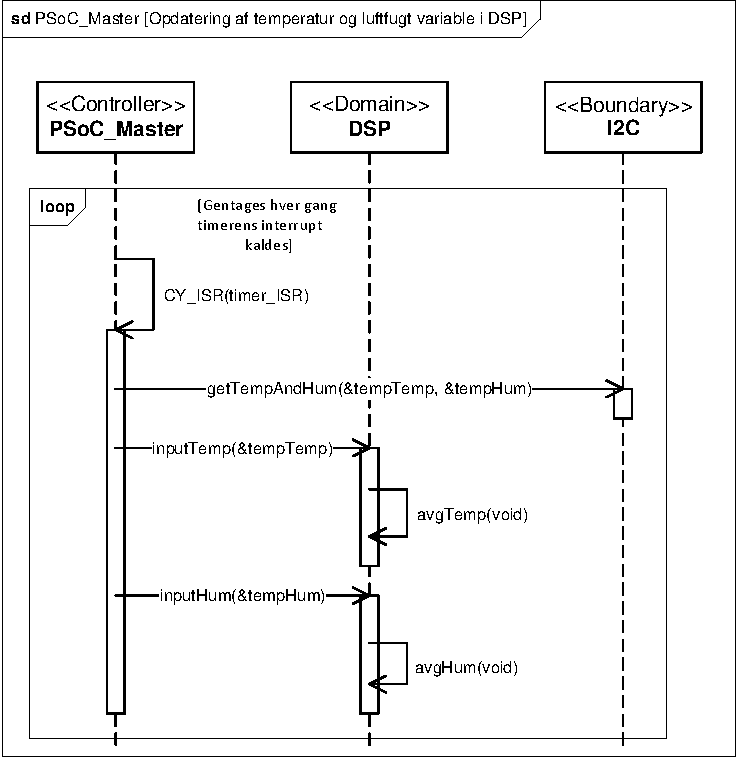
\includegraphics[scale=1]{../fig/sd_PSoC_master_update_sensor_values}
\caption{Sekvensdiagram over opdatering af sensorer.}
\label{fig:sd_PSoC_master_sensor}
\end{figure}

\begin{figure}[h]
\centering
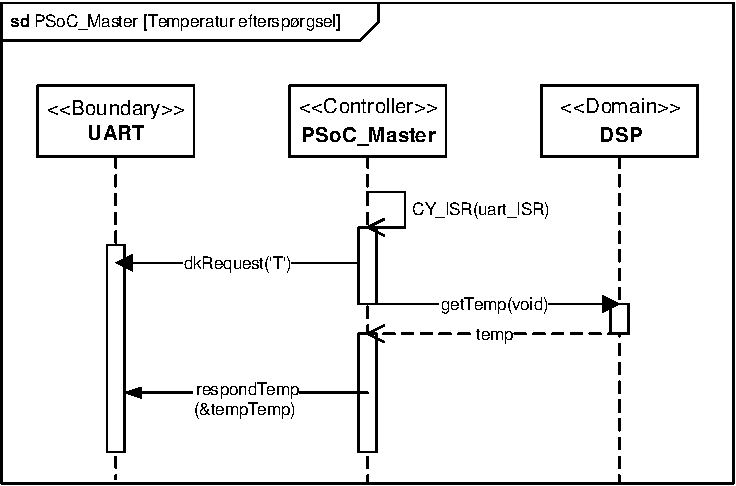
\includegraphics[scale=1]{../fig/sd_PSoC_master_tempreq}
\caption{Sekvensdiagram over forespørgsel af temperatur.}
\label{fig:sd_PSoC_master_tempreq}
\end{figure}

\begin{figure}[h]
\centering
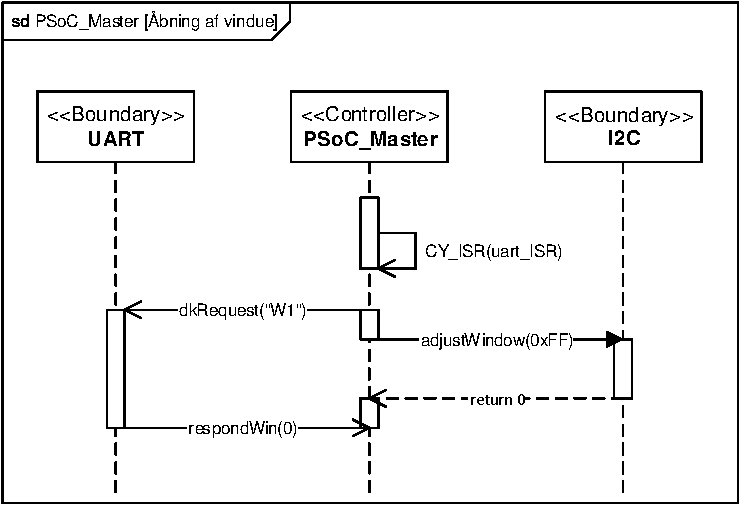
\includegraphics[scale=1]{../fig/sd_PSoC_master_open_window}
\caption{Sekvensdiagram over åbning af vindue.}
\label{fig:sd_PSoC_master_window}
\end{figure}



\clearpage
\section{Breakoutboards} \label{sec:breakoutboards}

Da AutoGreen er tiltænkt at skulle monitorere temperatur, luftfugtighed og lysintensitet, blev der valgt nogle sensorer der kunne foretage målinger af disse variable. 

Temperatur- og luftfugtighedssensoren som blev valgt var en \textit{HONEYWELL S\&C  HIH6030-021-001} \cite{lib:TempHum_DS}. Sensoren følger en standard \IIC-protokol og det er nødvendigt at tage hensyn til \IIC-klokkens hastighed samt spændingen på \IIC-bussen, så det er muligt for alle enheder på bussen at kommunikere. Fra producenten har sensoren fået en standard adresse, som skal bruges til kommunikation med enheden.

Lyssensoren der blev valgt var en \textit{Intersil ISL29010IROZ}\cite{lib:LightSens}. Lysfølsomheden kan ændres i sensoren ved at ændre en reference vha. forskellige modstandsstørrelser. Intensiteten af lyset måles i lumen, og sensoren kan måle fra 0 til 128.000 lumen, hvilket passer fint til drivhuset, som kan stå både i mørke og i stærk sollys. Som udgangspunkt oplyser databladet at sensoren fungerer bedst som vist i multisimdiagrammet i Figur \ref{fig:temp_fugt_lys_design}.

Størrelsen på sensorene gør dem meget svære at arbejde med, så der blev designet et breakoutboard til hver sensor. 
Både Temp/Luftfugt og Lyssensoren er af SOIC typen og meget små, så der er anvendt Multisim og Ultiboard til design af breakoutboards, så interfacing med sensorerne blev gjort væsentligt nemmere. Kredsløbene for breakout boards kan ses i Figur \ref{fig:temp_fugt_lys_design}. 

\begin{figure}[h]
\centering
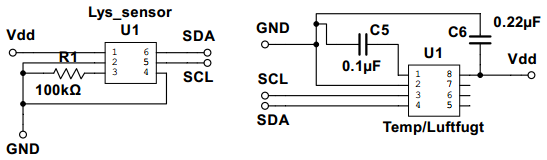
\includegraphics[trim=0 0 0 0, clip=true]{../fig/TempOgLys.png}
\caption{Design af temp/luftfugtsensor og lyssensor breakoutboards.}
\label{fig:temp_fugt_lys_design}
\end{figure}

Alle komponenters værdier fra billederne er taget fra sensorernes datablade.

\clearpage
\section{Aktuator Design (Henrik og Morten)}

Dette afsnit omhandler design af blokken Aktuator. Den opdeles i underblokkene Varmelegeme, Blæsere, Vinduesmotor og PSoC4.

\subsection{Varmelegeme}

\begin{figure}[h]
\centering 
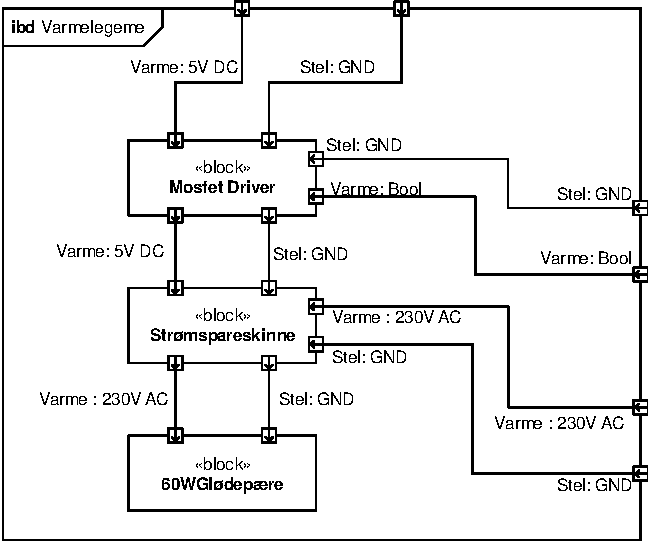
\includegraphics[width={\textwidth-5cm}, trim=0 0 0 0, clip=true] {../fig/ibd_varmelegeme.pdf}
\caption{IBD for underblokken Varmelegeme i Aktuator}
\label{fig:ibd_varmelegeme}
\end{figure}

Ovenstående diagram (Figur \ref{fig:ibd_varmelegeme}) viser interne forbindelser i underblokken Varmelegeme i Aktuator. 
For at undgå håndtering af 230V AC, består underblokken af en USB strømspareskinne, så selve varmelegemet (1-3 stk. 100W Glødepære) kan tændes og slukkes med et 5V DC signal. 
Antallet af tilkoblede glødepærer bestemmes under senere tests.

Aktuatorens SW er designet således at der nemt kan opgraderes til PWM styring af varmelegemet. 
Dette viser sig desværre at være umuligt med denne opstilling, da USB strømspareskinnen indeholder et mekanisk relæ; det er ikke muligt at opnå en frekvens hvor lyset ikke blinker. 
Dette vil sandsynligvis resultere i en sprunget glødepære.
En mulig løsning på problemet kunne være at tænde og slukke de 230V AC direkte med Mosfet transistoren, men vi må ikke håndtere så høje spændinger. 
En anden mulig løsning er at anvende for eksempel 12V glødepærer i stedet. Der skal dog nok temmelig mange til for at opnå samme effekt. 

Såfremt det senere vælges at opgradere til PWM styring, skal man tage højde for - eller se bort fra - at effekten ikke er lineært sammenhængende med dytucyclen. Dette skyldes dels at effekt har en sammenhæng med kvadratet af strømmen, dels at modstanden i glødetråden afhænger af temperaturen. 

\clearpage

\begin{figure}[h]
\centering 
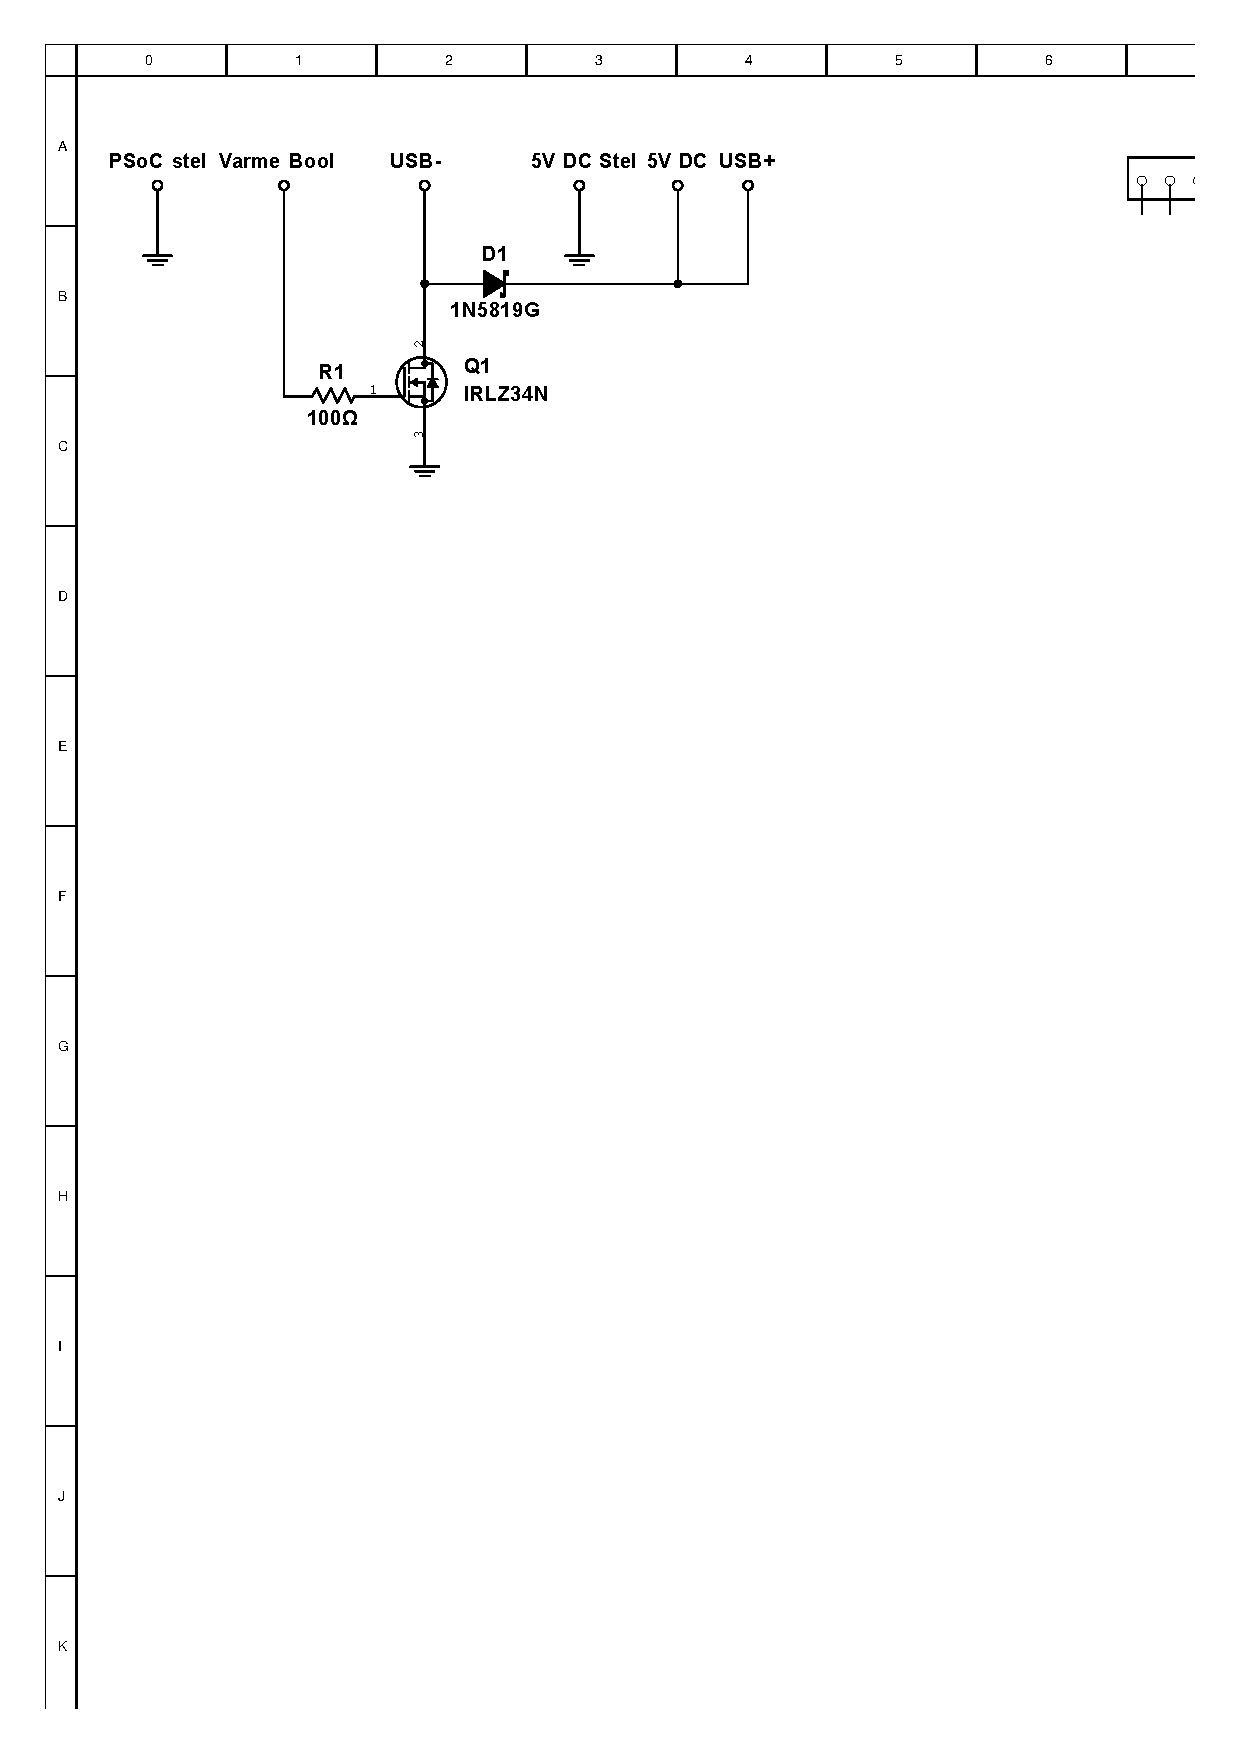
\includegraphics[width={\textwidth-5cm}, trim= 50 610 220 70, clip=true] {../fig/multisim_varmelegeme_mosfetdriver.pdf}
\caption{Kredsløb for Mosfet Driver i underblokken Varmelegeme}
\label{fig:multisim_varmelegeme_mosfetdriver}
\end{figure}

Når Varme Bool på Figur \ref{fig:ibd_varmelegeme} går høj, lukker mosfet transistoren, og tilslutter derved stel til USB Strømspareskinnen; varmelegemet forsynes med 230V AC. 
Når Varme Bool går lav, åbner mosfet transistoren, og derved afbrydes stel til Strømspareskinnen; varmelegemet forsynes ikke.  

D1 er er indsat for at sikre transistoren mod peakspændinger fra USB skinnen, når den slukkes. Dette er sandsynligvis ikke nødvendigt, men da vi ikke har indblik i hvordan USB strømspareskinnen rent faktisk virker, er dioden indsat for en sikkerheds skyld. 

Modstanden R1 er en beskyttelsesmodstand, som beskytter PSoC4, hvis Mosfet transistoren brændes af. 

\clearpage

\subsection{Blæsere}

\begin{figure}[h]
\centering 
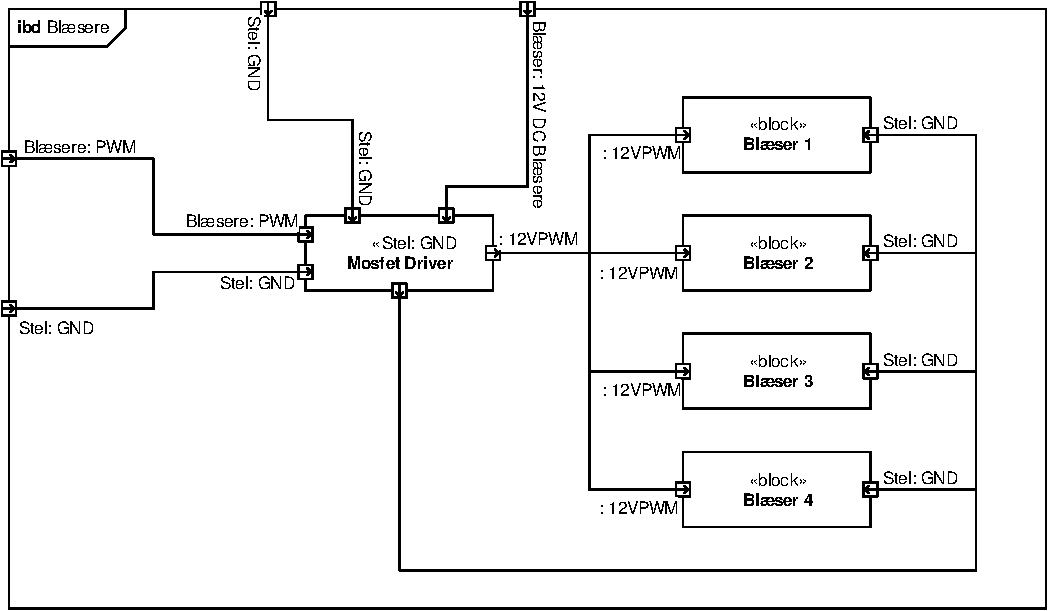
\includegraphics[width={\textwidth}, trim=0 0 0 0, clip=true] {../fig/ibd_blaesere.pdf}
\caption{IBD for underblokken Blæsere i Aktuator}
\label{fig:ibd_blaesere}
\end{figure}

Figur \ref{fig:ibd_blaesere} viser interne forbindelser i underblokken Blæsere, der består af en Mosfet Driver og fire 12V blæsere. 
To af blæserne er monteret således at luft blæses ind i drivhuset, mens de to øvrige blæsere blæser luft ud af drivhuset. 
Det forventes at en dutycycle på 100\% udskifter al luft i drivhuset på meget kort tid; dutycyclen for 'tændte blæsere' bestemmes ved praktiske forsøg under realisering af underblokken. 

Ved praktiske forsøg, konstateredes det, at en dutycyce på 50\% er et fornuftigt maximum. Det konstateredes desuden, at blæserne skal startes på maximum (dutycycle 50\%) for at komme i gang. 
Hvis der startes med en mindre dutycycle, opnår motoren ikke inerti nok til at begynde dreje. 
Begge dele implementeres i SW. 

\clearpage
 
\begin{figure}[h]
\centering 
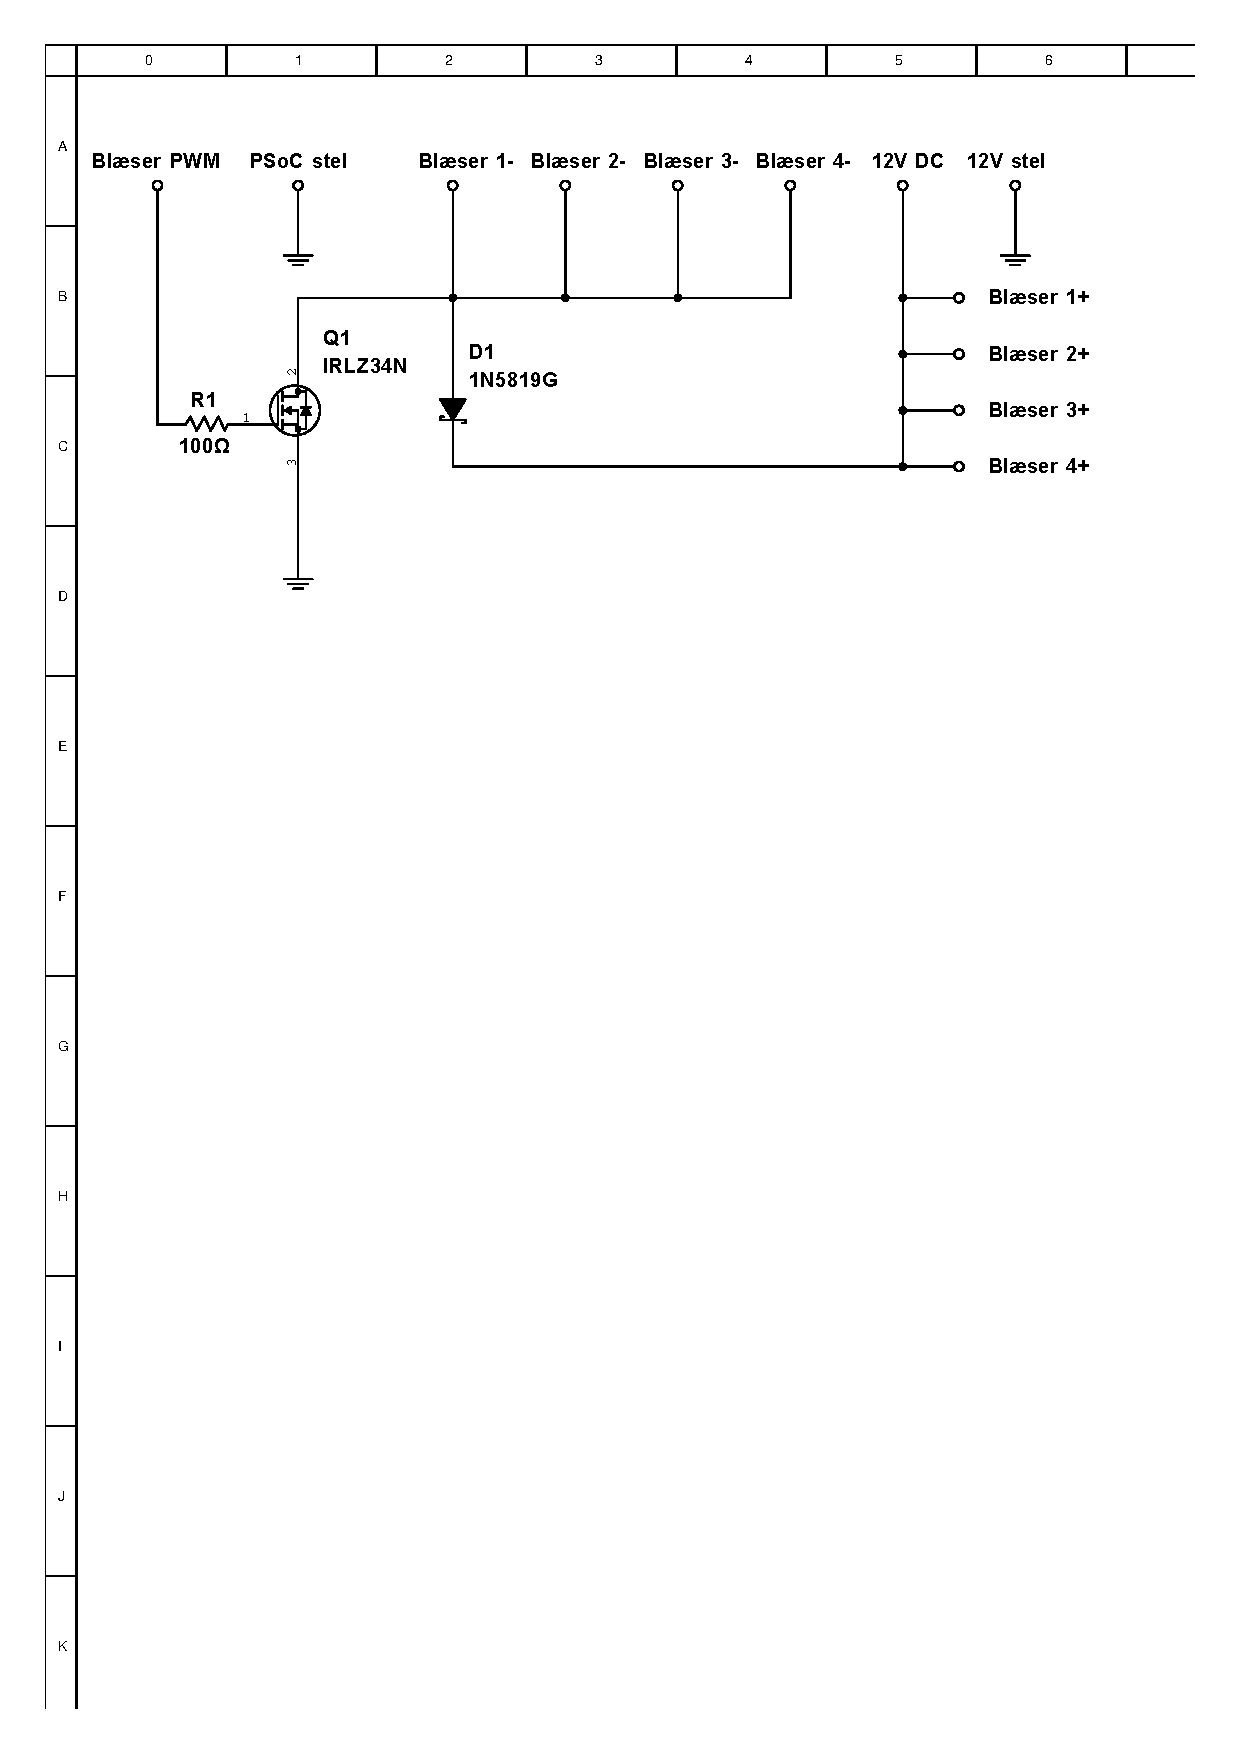
\includegraphics[width={\textwidth}, trim= 40 550 70 70, clip=true] {../fig/multisim_blaesere_mosfetdriver.pdf}
\caption{Kredsløb for Mosfet Driver i underblokken Blæsere}
\label{fig:multisim_blaesere_mosfetdriver}
\end{figure}

Mosfet Driveren til Blæsere på Figur \ref{fig:multisim_blaesere_mosfetdriver} fungerer i princippet på samme måde som Mosfet Driver for Varmelegeme (Figur \ref{fig:multisim_varmelegeme_mosfetdriver}).
Der er blot tilsluttet fire blæsere, der alle styres vha. den samme transistor. 

\clearpage

\subsection{Vinduesmotor}

\begin{figure}[h]
\centering 
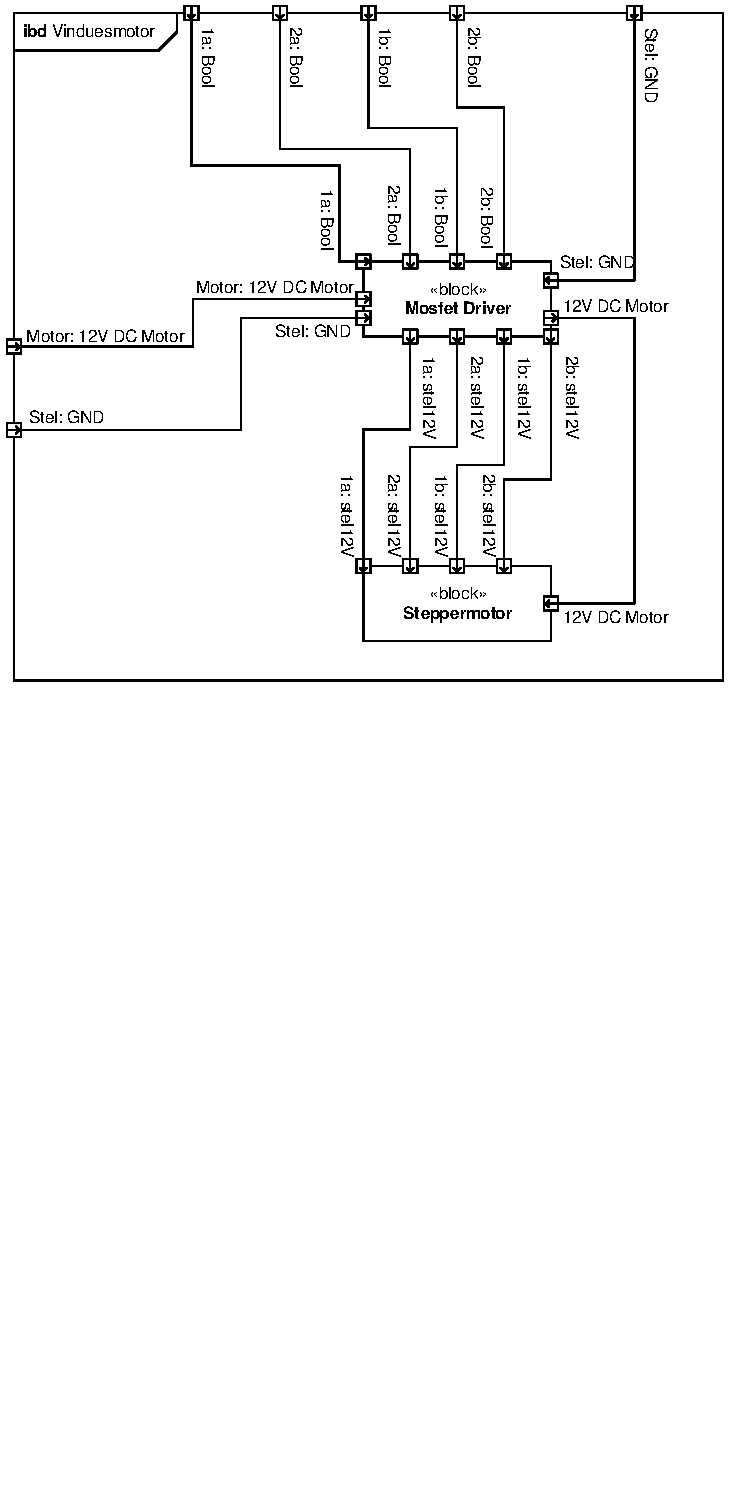
\includegraphics[width={\textwidth}, trim=0 390 0 0, clip=true] {../fig/ibd_vinduesmotor.pdf}
\caption{IBD for underblokken Vinduesmotor i Aktuator}
\label{fig:ibd_vinduesmotor}
\end{figure}

Ovenstående diagram (Figur \ref{fig:ibd_vinduesmotor}) viser interne forbindelser i underblokken Vinduesmotor, der består af en Steppermotor og en Mosfetdriver. 
Der åbnes og lukkes for mosfet transistorer i Mosfet Driveren vha. 3,3V signaler fra PSoC4, og derved forsynes Steppermotor med 12V DC. 
\\\\
Mosfet Driveren til Vinduesmotor på Figur \ref{fig:multisim_vinduesmotor_mosfetdriver} side \pageref{fig:multisim_vinduesmotor_mosfetdriver} fungerer i princippet på samme måde som Mosfet Driver for Blæsere (Figur \ref{fig:multisim_blaesere_mosfetdriver}).
Der er dog den forskel, at de fire signaler styres af hver deres transistor, da de ikke alle skal åbne og lukke samtidigt. 

\begin{figure}[h]
\centering 
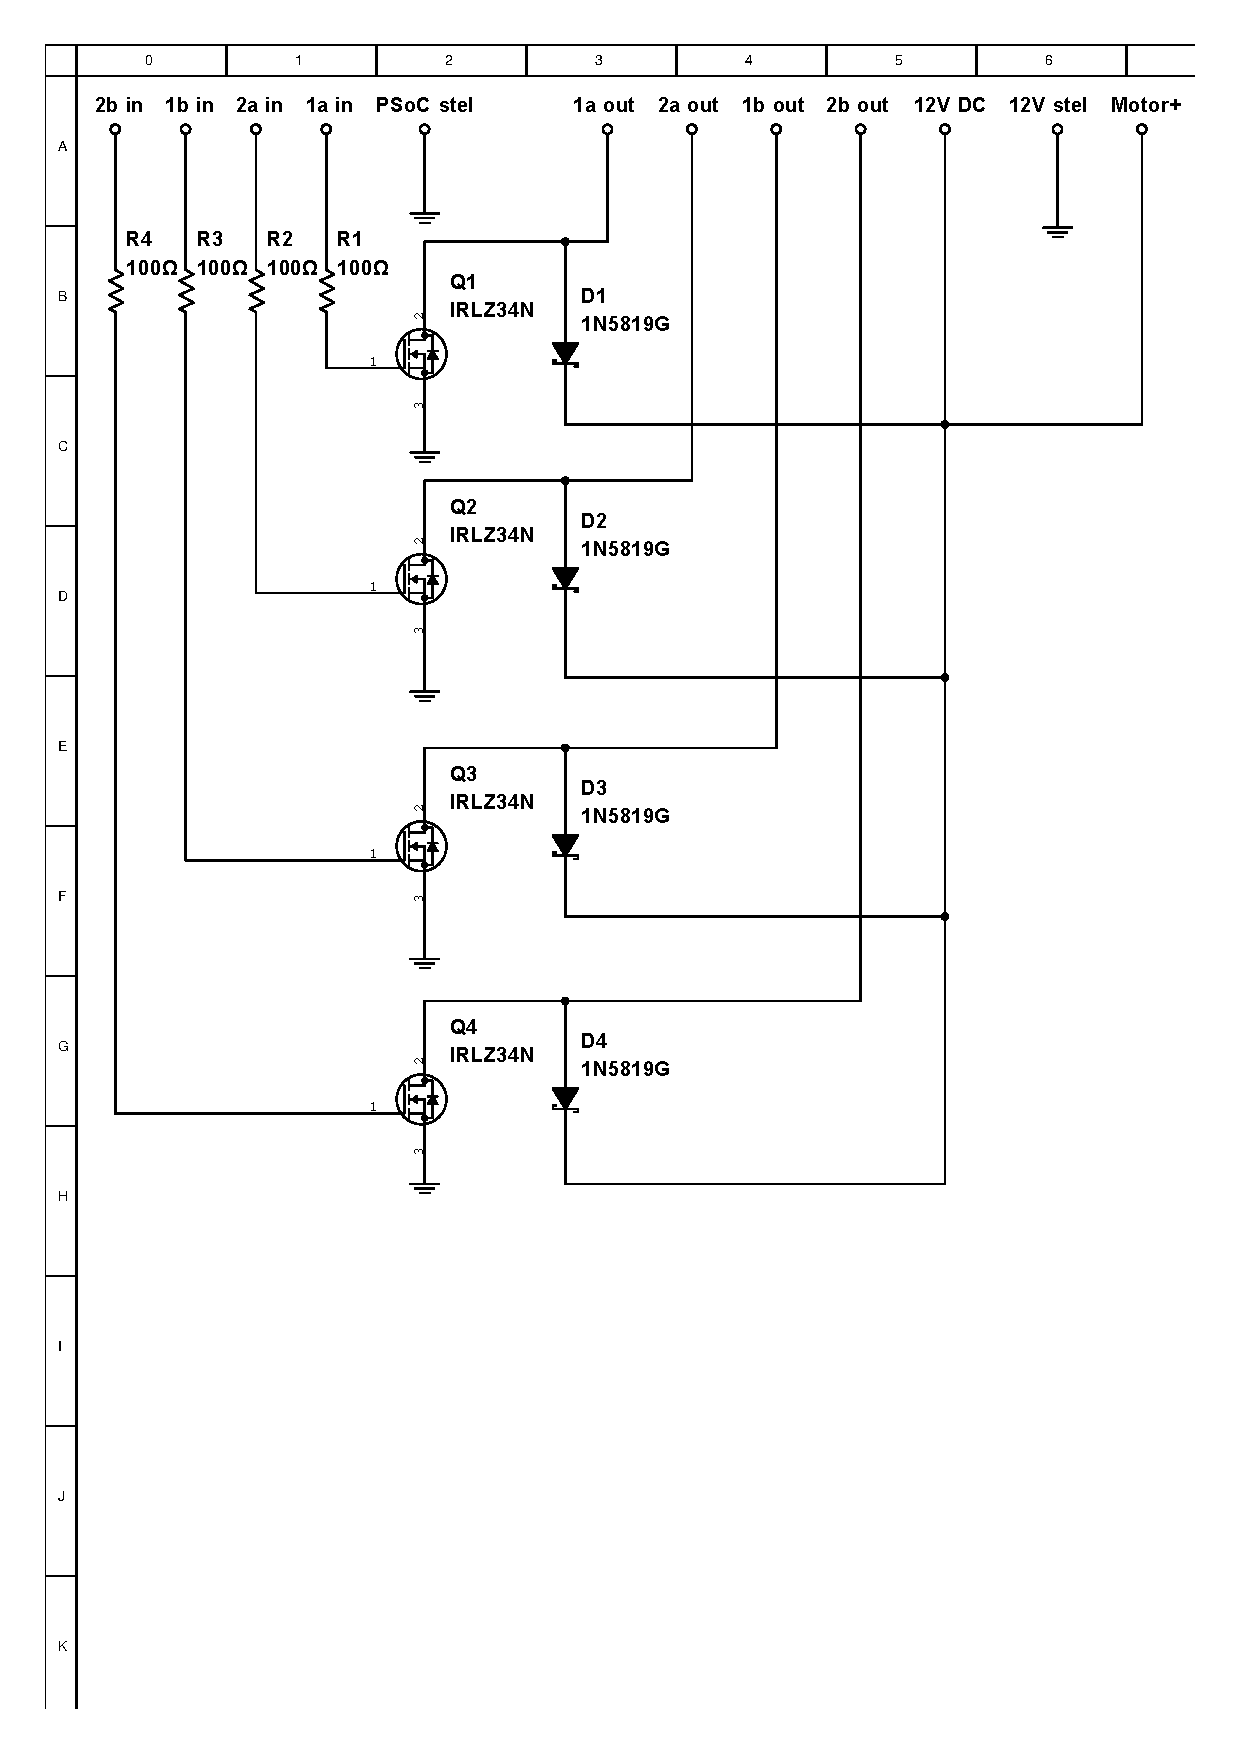
\includegraphics[width={\textwidth}, trim= 40 260 0 40, clip=true] {../fig/multisim_vinduesmotor_mosfetdriver.pdf}
\caption{Kredsløb for Mosfet Driver i underblokken Vinduesmotor}
\label{fig:multisim_vinduesmotor_mosfetdriver}
\end{figure}

\clearpage

\subsection{PSoC4}

\begin{figure}[h]
\centering 
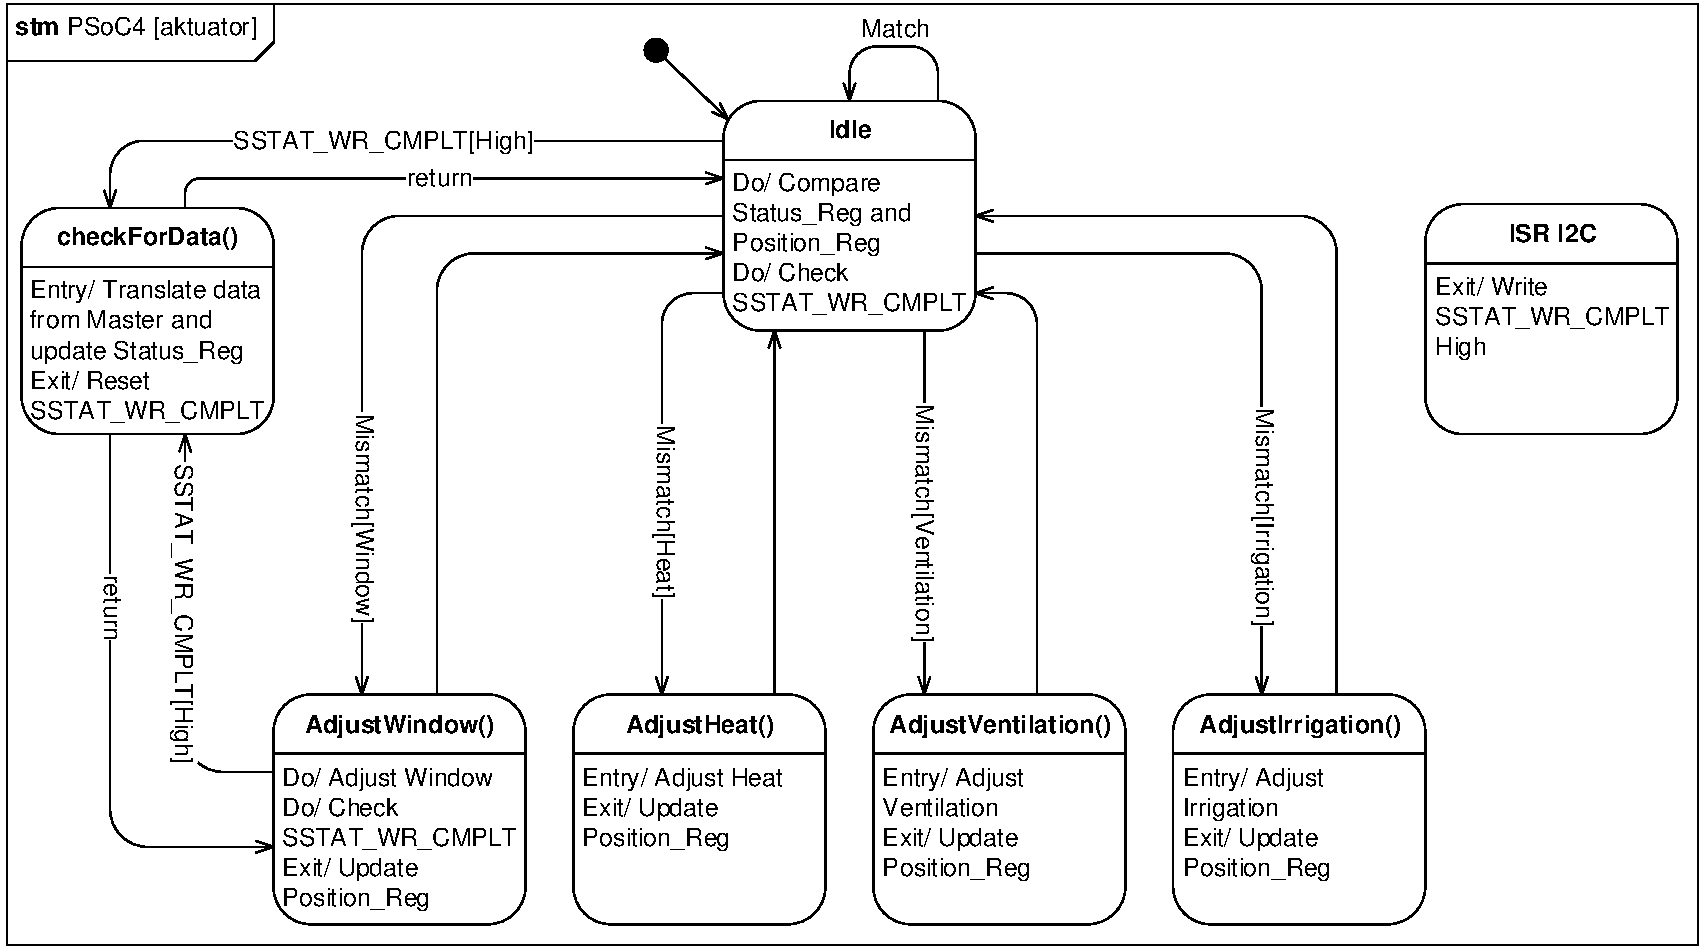
\includegraphics[width={\textwidth}, trim=0 0 0 0, clip=true] {../fig/stm_psoc_aktuator.pdf}
\caption{State Machine for software på underblokken PSoC4 i Aktuator}
\label{fig:stm_psoc_aktuator}
\end{figure}

Ovenstående diagram (Figur \ref{fig:stm_psoc_aktuator}) viser en state machine for software i underblokken PSoC4 i blokken Aktuator. 

Koden gentager tjek af om ønsket indstilling, af aktuatorer stemmer overens med aktuatorernes aktuelle indstilling og retter dette, såfremt det ikke er tilfældet. 
Denne rutine kan til enhver tid afbrydes af interrupt fra I2C bussen, der opdaterer slave write complete registeret (SSTAT\_WR\_CMPLT) fra lav til høj. Dette medfører at checkForData aktiveres som opdaterer ønskede indstillinger af aktuatorer. Herefter vil rutinen genoptages.
 
Ønskede indstillinger er gemt i registret Status\_Reg, mens aktuelle indstillinger er gemt i Position\_Reg.
 
Ved opdaterering af aktuatorer er den priorterede rækkefølge: Varme, blæsere, vanding og vindue. 
Vinduet er sidst i rækkefølgen, da det tager lang tid at åbne eller lukke. Koden for åbning eller lukning af vindue skrives således, at slave write complete registeret løbende tjekkes. Hvis dette register er højt vil indstillinger af aktuatorer opdateres, og derefter fortsætte fra vinduets position med de nye indstillinger.
Derved undgås det, at vinduet fx skal lukke helt, inden det åbnes, hvis disse to kommandoer modtages med meget kort mellemrum. 

\subsection{Drivers til PSoC4}
Dette afsnit beskriver drivere for opdatering af aktuatorer. 
Disse drivere er opdelt i Varme, Blæsere, Vanding, Vinduesmotor og checkForData. 
Derved kan systemet nemt opdateres, hvis der ændres på styringen af en bestemt aktuator. 
Alle drivere består af en header fil med prototyper og en source fil med implementeringer.

\subsubsection{Driver Varme}
Denne driver indeholder en funktionalitet, der har til formål at tænde eller slukke varmelegemet, samt opdatere aktuatorens bits i Position\_Reg. 
Dette sker ved at sætte en pin på PSoC4 hhv. høj eller lav; det gøres vha. PWM, da der så senere er nem mulighed for at opgradere styringen af varmelegemet til PWM styring. 

\subsubsection{Driver Blæsere}
Driveren for Blæsere har til formål at starte eller stoppe de fire blæsere i drivhuset, samt opdatere aktuatorens bits i Position\_Reg.
Dette sker ved at sende et PWM signal ud på en pin på PSoC4. 

\subsubsection{Driver Vanding}
Denne driver har til formål at aktivere eller deaktivere aktuatorer for vanding, samt opdatere aktuatorens bits i Position\_Reg. 
Dette sker ved at sætte 6 forskellige pins på PSoC4 hhv. høj eller lav. 

\subsubsection{Driver Vinduesmotor}
Driveren for vinduesmotoren har til formål at åbne eller lukke vinduet, samt opdatere aktuatorens bits i Position\_Reg. 
Antallet af omdrejninger for at åbne vinduet bestemmes under realisering ved praktiske forsøg. 
Driveren skal sammenligne Position\_Reg med Status\_Reg for hver omgang steppermotoren kører. 
Derved undgås det fx, at vinduet er nødt til at åbne helt inden det lukkes, hvis disse to kommandoer modtages hurtigt efter hinanden. 
Koden skrives således at det er nemt senere at opdatere driveren, så vinduet kan indstilles i flere trin mellem åbent og lukket. 

\subsubsection{Driver checkForData}
Denne driver har til formål at opdatere Status\_Reg. Der er mulighed for at kalde denne fra Idle tilstand og under AdjustWindow.
Driveren kaldes kun i det tilfælde, at I2C bussen har kaldt et interrupt, hvilket medfører opdatering af slave write complete registeret fra lav til høj.

\clearpage	
\section{Strømforsyning Design} \label{sec:Stroemforsyning_Design}

Som nævnt i systemarkitekturen forsyner strømforsyningen øvrig HW i systemet, undtagen selve varmelegemet og DevKit8000, der forsynes med 230V AC, og sensorerne, der forsynes med VEE (3.3V DC) fra PSoC Master.

Strømforsyningen forsynes med 12V DC max. 3A fra en laboratorieforsyning jf. Signalbeskrivelser på Tabel \ref{tbl:signalbeskriv} på side \pageref{tbl:signalbeskriv}. 
Alternativt kan anvendes en 12V transformer, der kobles til 230V AC. 

Strømforsyningen skal have 12V DC udgange til motor og blæsere, USB udgange med VDD til PSoC4 Pioneer Kits og en VDD udgang til USB strømspareskinnen.

\begin{figure}[h]
\centering 
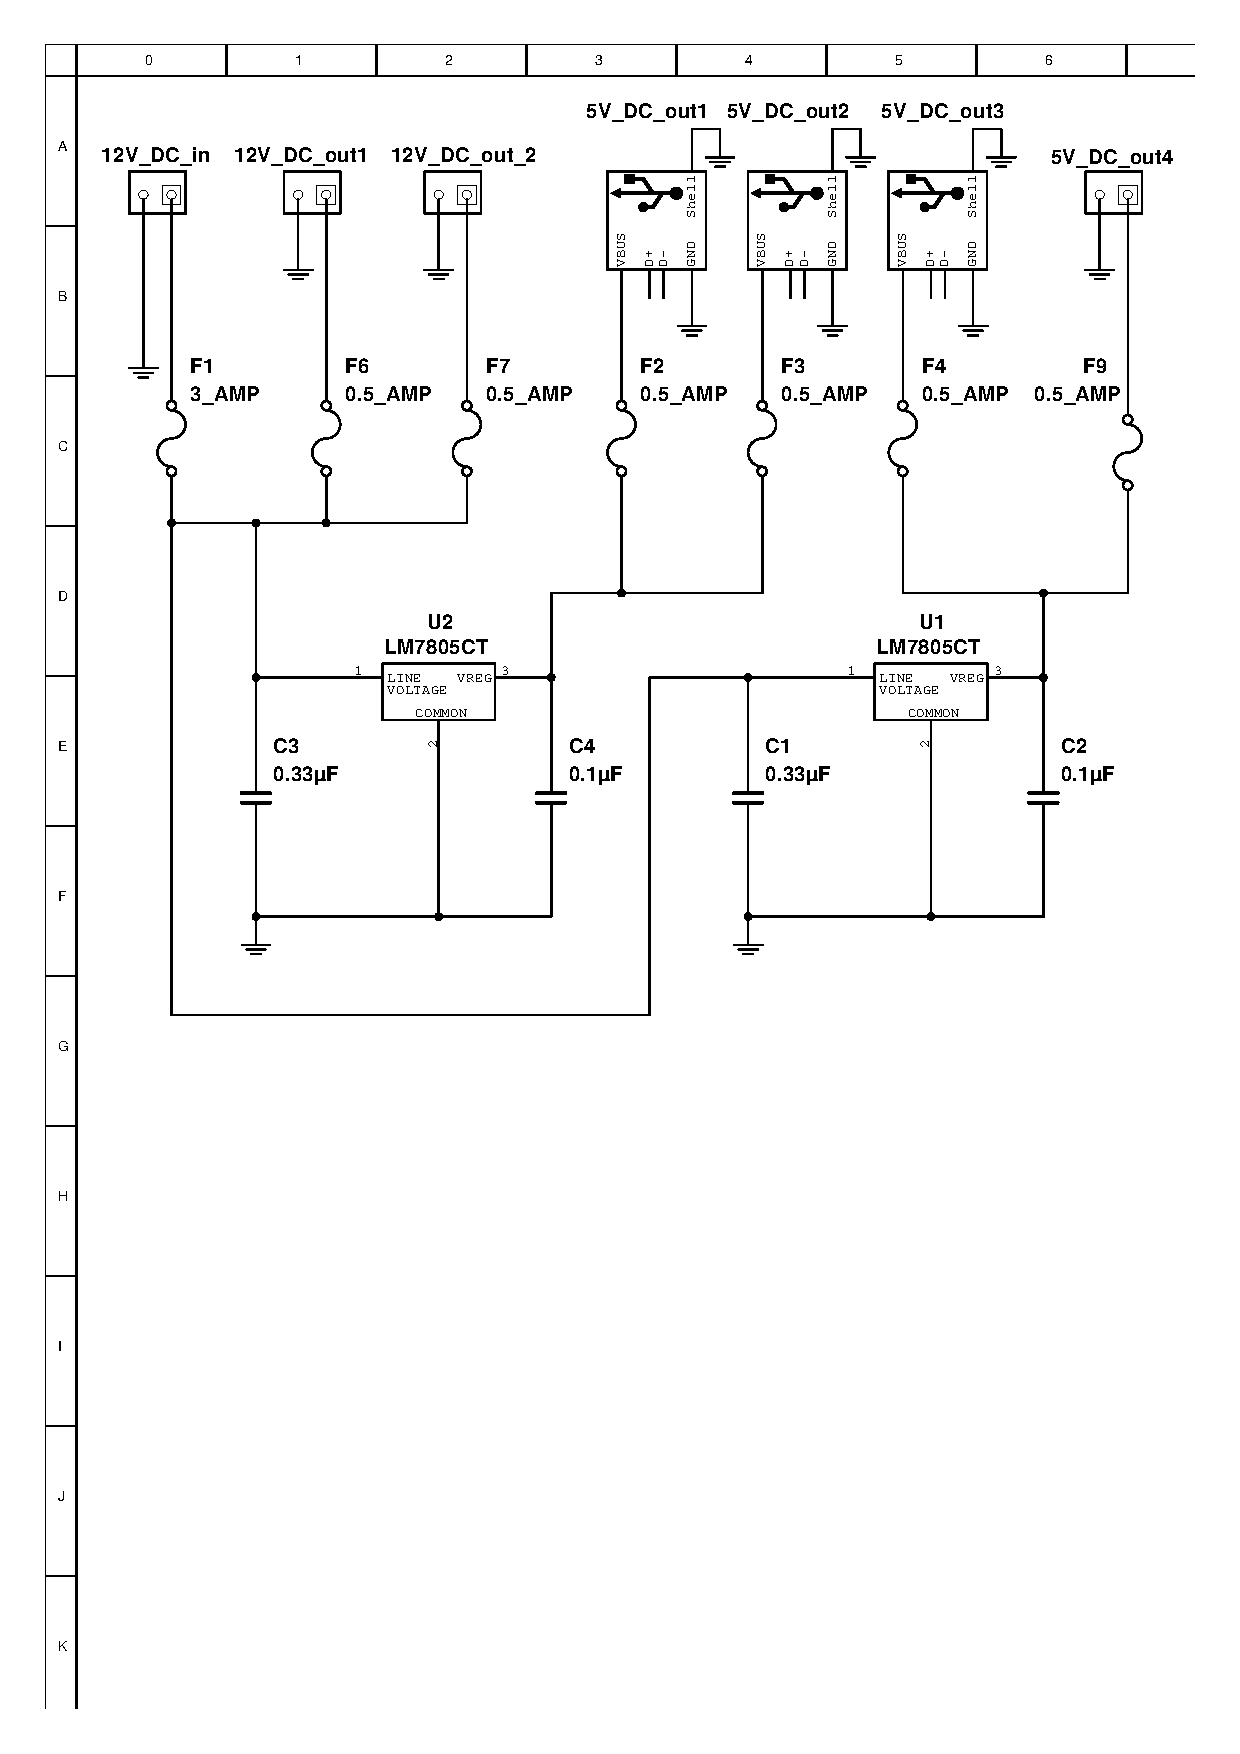
\includegraphics[width={\textwidth}, trim=50 350 30 40, clip=true] {../fig/multisim_stroemforsyning.pdf}
\caption{Diagram for blokken Strømforsyning}
\label{fig:multisim_stroemforsyning}
\end{figure}

Figur \ref{fig:multisim_stroemforsyning} viser Multisim diagram for designet af blokken Stroemforsyning. 
De enkelte komponenter og overvejelser herom gennemgås nedfor. 

\clearpage

12V DC in (VCC) trækker som sagt max. 3A, derfor monteres denne med en sikring på denne størrelse. 

12V DC out1 udgangen til motor trækker max. 500 mA jf. databladet \cite{lib:UHD2_DS} side 38, derfor monteres den med en sikring på 500 mA. 

De fire blæsere trækker hver især max. 140 mA ved fuld styrke jf. påtrykt værdi på selve blæserne. 
Implementeringen af koden i blokken Aktuator er lavet således, at blæserne maximalt kommer til at køre med en dutycycle på 50\%. 
Derfor monteres ligeledes en sikring på 500 mA til de fire blæsere. 

Ved en praktisk undersøgelse af USB skinnen konstateredes det, at USB indgangen trækker ca. 400 mA, når relæet er slået til, derfor monteres der også en 500 mA sikring på denne udgang. 

Der anvendes to spændingregulatorer LM7805, som begrænser 12V DC til 5V DC. 
De kan hver især levere 1A, derfor anvendes to stk. 
De monteres med afkoblinger til stel på ben 1 og 3 jf. standardapplikationen på side 1 i databladet \cite{lib:LM7805_DS}.

\clearpage


\section{Jordfugt Design} \label{sec:Jordfugt_Design}

Dette afsnit omhandler design af blokken Jordfugt, der består af et PSoC4 Pioneer kit og 0-6 jordfugtsensorer. 

\begin{figure}[h]
\centering 
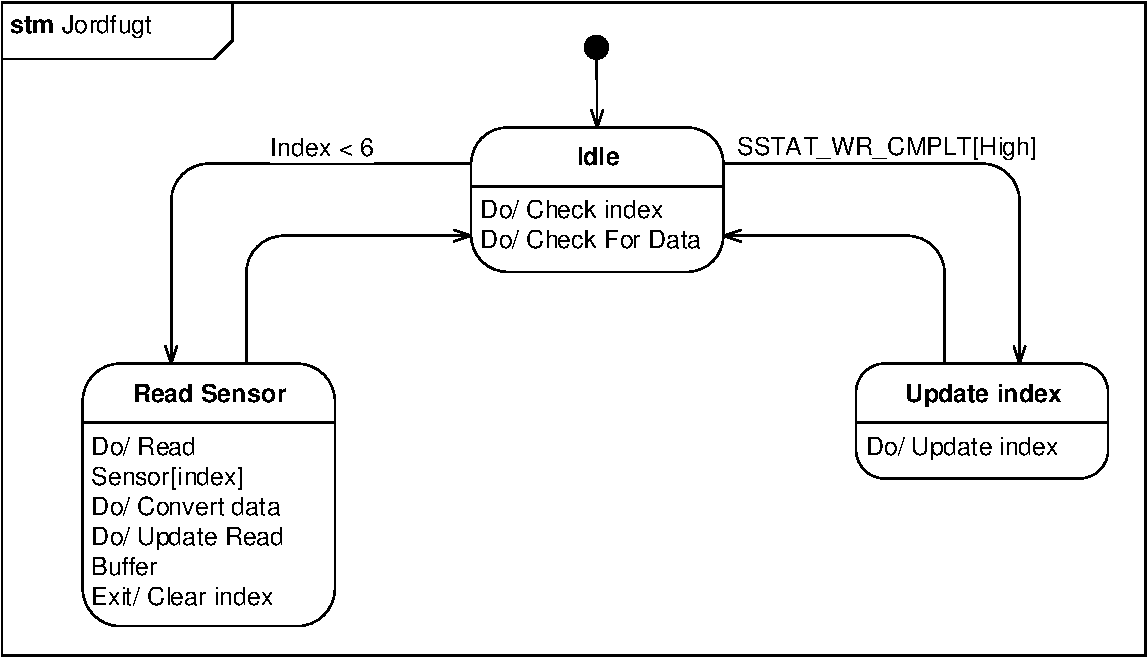
\includegraphics[width={\textwidth}, trim=0 0 0 0, clip=true] {../fig/stm_jordfugt.pdf}
\caption{State Machine for SW på PSoC4 i blokken Jordfugt}
\label{fig:stm_jordfugt}
\end{figure}

Ovenstående figur (Figur \ref{fig:stm_jordfugt}) viser en state machine for SW i PSoC4 i blokken Jordfugt.
 
PSoC'en står hele tiden og poller på om der er modtaget data, og om en indexvariabel er mindre end 6, som er det maximale antal jordfugtsensorer, der kan tilkobles.

Såfremt der er modtaget data via \IIC komminukationen, opdateres index variablen til det sensornummer, der er modtaget. 

Såfremt index variablem er mindre end 6, læses der på den tilhørende sensor, data konverteres til et tal mellem 1 - 100, og read bufferen opdateres med den læste værdi. 

\mbox{}

Der er i forbindelse med brugen af sensoren lavet en støjundersøgelse i faget Mixed Signal Elektronik. 
Se journalen \cite{lib:MSE_06} for nærmere info. 
I AutoGreen anvendes jordfugtsensoren på en noget simplere måde end i øvelsen, se afsnittet om implementering af blokken Jordfugt for nærmere info.

\clearpage